\documentclass[a4paper,10pt,twoside]{article}

\usepackage[top=1in, bottom=1in, left=1in, right=1in]{geometry}
\usepackage[utf8]{inputenc}
\usepackage[spanish,es-ucroman,es-noquoting]{babel}
\usepackage{setspace}
\usepackage{fancyhdr}
\usepackage{lastpage}
\usepackage{amsmath}
\usepackage{amsfonts}
\usepackage{amsthm}
\usepackage{verbatim}
\usepackage{graphicx}
\usepackage{float}
\usepackage{algpseudocode}
\usepackage{enumitem} % Provee macro \setlist
\usepackage[toc, page]{appendix}


%%%%%%%%%% Configuración de Fancyhdr - Inicio %%%%%%%%%%
\pagestyle{fancy}
\thispagestyle{fancy}
\lhead{Trabajo Práctico 1 · Algoritmos y Estructuras de Datos III}
\rhead{Lovisolo · Petaccio · Rossi}
\renewcommand{\footrulewidth}{0.4pt}
\cfoot{\thepage /\pageref{LastPage}}

\fancypagestyle{caratula} {
   \fancyhf{}
   \cfoot{\thepage /\pageref{LastPage}}
   \renewcommand{\headrulewidth}{0pt}
   \renewcommand{\footrulewidth}{0pt}
}
%%%%%%%%%% Configuración de Fancyhdr - Fin %%%%%%%%%%


%%%%%%%%%% Configuración de Algorithmic - Inicio %%%%%%%%%%
% Entorno propio para customizar la presentación del pseudocódigo
\newenvironment{pseudo}[1][]{%
    \vspace{0.5em}%
    \begin{algorithmic}%
}
{%
    \end{algorithmic}%
    \vspace{0.5em}%
}

% Conectivo 'in' para usar así: \ForAll{$foo$ \In $bar$}
\newcommand{\In}{\textbf{in} }

% Conectivo 'to' para usar así: \For{$i = 1$ \In $n$}
\newcommand{\To}{\textbf{to} }

% Complejidades
\newcommand{\Ode}[1]{\hfill $O(#1)$}
%%%%%%%%%% Configuración de Algorithmic - Fin %%%%%%%%%%


%%%%%%%%%% Miscelánea - Inicio %%%%%%%%%%
% Evita que el documento se estire verticalmente para ocupar el espacio vacío
% en cada página.
\raggedbottom

% Deshabilita sangría en la primer línea de un párrafo.
\setlength{\parindent}{0em}

% Separación entre párrafos.
\setlength{\parskip}{0.5em}

% Separación entre elementos de listas.
\setlist{itemsep=0.5em}

% Asigna la traducción de la palabra 'Appendices'.
\renewcommand{\appendixtocname}{Apéndices}
\renewcommand{\appendixpagename}{Apéndices}
%%%%%%%%%% Miscelánea - Fin %%%%%%%%%%


\begin{document}


%%%%%%%%%%%%%%%%%%%%%%%%%%%%%%%%%%%%%%%%%%%%%%%%%%%%%%%%%%%%%%%%%%%%%%%%%%%%%%%
%% Carátula                                                                  %%
%%%%%%%%%%%%%%%%%%%%%%%%%%%%%%%%%%%%%%%%%%%%%%%%%%%%%%%%%%%%%%%%%%%%%%%%%%%%%%%


\thispagestyle{caratula}

\begin{center}


\includegraphics[height=2cm]{DC.png} 
\hfill

\includegraphics[height=2cm]{UBA.jpg} 

\vspace{2cm}

Departamento de Computación,\\
Facultad de Ciencias Exactas y Naturales,\\
Universidad de Buenos Aires

\vspace{4cm}

\begin{Huge}
Trabajo Práctico 1
\end{Huge}

\vspace{0.5cm}

\begin{Large}
Algoritmos y Estructuras de Datos III
\end{Large}

\vspace{1cm}

Segundo Cuatrimestre de 2013

\vspace{4cm}

\begin{tabular}{|c|c|c|}
\hline
Apellido y Nombre & LU & E-mail\\
\hline
Leandro Lovisolo      & 645/11 & leandro@leandro.me\\
Lautaro José Petaccio & 443/11 & lausuper@gmail.com\\
Lucas Rossi           & 705/11 & lucasrossi20@gmail.com\\
\hline
\end{tabular}

\end{center}

\newpage


%%%%%%%%%%%%%%%%%%%%%%%%%%%%%%%%%%%%%%%%%%%%%%%%%%%%%%%%%%%%%%%%%%%%%%%%%%%%%%%
%% Índice                                                                    %%
%%%%%%%%%%%%%%%%%%%%%%%%%%%%%%%%%%%%%%%%%%%%%%%%%%%%%%%%%%%%%%%%%%%%%%%%%%%%%%%


\tableofcontents

\newpage


%%%%%%%%%%%%%%%%%%%%%%%%%%%%%%%%%%%%%%%%%%%%%%%%%%%%%%%%%%%%%%%%%%%%%%%%%%%%%%%
%% Introducción                                                              %%
%%%%%%%%%%%%%%%%%%%%%%%%%%%%%%%%%%%%%%%%%%%%%%%%%%%%%%%%%%%%%%%%%%%%%%%%%%%%%%%


\section{Introducción}

En el presente trabajo estudiamos tres problemas algorítmicos, proponemos soluciones para los mismos respetando sus requerimientos de complejidad temporal y analizamos empíricamente los tiempos de ejecución de sus implementaciones en lenguaje C++.

La motivación de este trabajo es comparar las cotas temporales obtenidas del análisis teórico con las mediciones de tiempos de ejecución y extraer conclusiones de esta experimentación.

Sin más, presentamos los problemas estudiados a continuación.


%%%%%%%%%%%%%%%%%%%%%%%%%%%%%%%%%%%%%%%%%%%%%%%%%%%%%%%%%%%%%%%%%%%%%%%%%%%%%%%
%% Problema 1: Pascual y el correo                                           %%
%%%%%%%%%%%%%%%%%%%%%%%%%%%%%%%%%%%%%%%%%%%%%%%%%%%%%%%%%%%%%%%%%%%%%%%%%%%%%%%


\newpage

\section{Problema 1: Pascual y el correo}

Dada una secuencia de paquetes y un límite de peso, se nos pide calcular, la cantidad de camiones necesarios y sus pesos, para realizar el transporte de los mismos, utilizando el método del encargado de logística llamado Pascual, el cuál consiste en lo siguiente:

\begin{itemize}
\item Si un paquete excede el peso del camión cargado con menor peso, se pide un nuevo camión y se coloca el paquete.
\item Si el paquete no supera el peso del camión cargado de menor peso, se lo coloca en el camión de menor peso.
\end{itemize}

Se nos pide resolver el problema con una cota de complejidad temporal \textbf{estrictamente mejor} que $O(n^2)$.

\textbf{Ejemplos del problema y sus soluciones:}

\textbf{Entrada}: límite: 100 , peso de paquetes: 3 80 40 60. \\
\textbf{Salida}: 2 80 100. \\
El camión 1 recibe el primer paquete de 80. Al intentar luego colocar el paquete de 40 en este, no le es posible debido a que el límite es 100 y lo guarda en el camión 2, al que luego, se le suma el paquete de 60, el cuál no provoca que el límite sea superado al colocarse en este.\\

\textbf{Entrada}: límite: 100, paquetes: 0.\\
\textbf{Salida}: 0. \\
Al no haber paquetes no se utilizan comiones, sin importar el límite del mismo.

\subsection{Solución}

Sea $\langle p_1, \ldots, p_n \rangle$ la secuencia que contiene los pesos de los $n$ paquetes en orden de llegada, sea $\langle c_1, \ldots, c_m \rangle$ la secuencia en orden ascendente que contiene las cargas de los camiones en un determinado momento (inicialmente vacía) y sea $L$ el límite de carga de los camiones.

Para cada paquete $p_i$, cargamos el paquete en el camión con menor carga $c_1$ si la nueva carga no supera el límite $L$, o en caso contrario agregamos un nuevo camión $c_{m+1} = p_i$ a la secuencia, realizando las permutaciones necesarias para preservar el orden ascendente.

Luego de haber cargado todos los paquetes, devolvemos la secuencia con la carga de cada camión.

Para cumplir con los requerimientos de complejidad temporal, utilizamos una cola de prioridad min-heap en lugar de una secuencia para almacenar las cargas de cada camión.

\begin{pseudo}
	\State Tipo de dato Camion es Tupla $\langle$ id : entero, carga : entero  $\rangle$
    \Procedure{Pascual-y-el-correo}{$\langle p_1, \ldots, p_n \rangle, L$}
        \State $C \leftarrow$ nuevo min-heap de Camion, ordenado por carga   \Ode{1}
        \ForAll{$p$ \In $\langle p_1, \ldots, p_n \rangle$}    	
            \If{$C.tama\tilde{n}o = 0$}                         \Ode{1}
                \State $C.encolar(\langle 1 , p \rangle)$       \Ode{log(n)}
            \ElsIf{$C.siguiente() + p \leq L$}                  \Ode{1}
                \State $c : Camion \leftarrow C.siguiente()$   \Ode{1}
                \State $c.carga \leftarrow c.carga + p$			\Ode{1}
                \State $C.desencolar()$                         \Ode{log(n)}
                \State $C.encolar(c)$                           \Ode{log(n)}
            \Else
                \State $C.encolar(\langle C.tama\tilde{n}o(), p \rangle)$ \Ode{log(n)}
            \EndIf
        \EndFor

  		\State $Camiones \leftarrow$ Arreglo de camiones de C.tamaño()
        \ForAll{$i$ \In $\langle 1, \ldots,$ C.tamaño() $\rangle$}			
      		\State Camiones[i] $\leftarrow$ $C.siguiente()$		\Ode{1}
      		\State $C.desencolar()$								\Ode{log(n)}
        \EndFor
        
        \State $Ordenar(Camiones)$ (Ordenamiento por id)		\Ode{log(n)}
        \State \textbf{return} $Camiones$
    \EndProcedure
\end{pseudo}


\subsection{Complejidad}

Para realizar el algoritmo se utilizó la estructura de datos priority\_queue que pertenece a la \textit{STL}.

Las operaciones operaciones utilizadas fueron \textit{top()} que corresponde a \textit{siguiente()} con complejidad \textit{O(1)} y \textit{push()} y \textit{pop()} que corresponden a \textit{encolar()} y \textit{desencolar()} con complejidad \textit{O(log(n))}.

El algoritmo corre en tiempo $O(n*log(n))$, donde $n$ es la cantidad de paquetes.

Demostración: para cada uno de los $n$ paquetes, se realizan 1 ó 2 operaciones $O(log(n))$ sobre la cola de prioridad. Luego deducimos la complejidad total $n * O(log(n)) = O(n * log(n))$.


\subsection{Correctitud}
Sea m el paquete número m de la secuencia de paquetes recibida, con m-1 paquetes ubicados en camiones anteriormente, quiero ver si al ubicar el paquete m el algoritmo cumple con la metodología de ordenar paquetes de Pascual.

Al utilizar una \textbf{cola de prioridad} para almacenar los camiones, es posible asegurar que siempre se tendrá el camión menos cargado en cada llamada a \textbf{Siguiente}, corroborando el correcto funcionamiento de la consigna, la cuál describe que las comparaciones para elegir el destino del paquete se hacen con el camión de menor peso. 

Si la suma del peso del camión en la cabecera y el nuevo paquete m no superan el límite, se procede a desencolar del heap el camión, se le carga el nuevo paquete aumentando su peso y se lo encola nuevamente en el heap el cuál se encargará de dejar el nuevo camión con menos peso en la cabecera.

Si es requerido un nuevo camión, se crea uno nuevo con el peso del paquete m y se lo encola en el heap, nuevamente el heap se encargará de colocar el camión de menor peso en la cabecera.

\subsection{Experimentos computacionales}
\subsubsection{Verificación de correctitud}
Elegimos los siguientes casos para verificar la correctitud del programa:
\begin{enumerate}
	\item Entrada vacía, verifica el comportamiento del algoritmo ante la posibilida de no recibir ningún paquete en la entrada.
	\item Entrada con un único paquete, verifica el primer caso, el de tener el \textbf{min-heap} vacío.
	\item Entrada en la cual en algún camión se deba insertar más de un paquete. Esto verifica el caso del \textbf{else if} descripto en el pseudocódigo.
	\item Entrada en la cual algún camión no pueda contener el peso del nuevo paquete y deba pedir un nuevo camión. Esto verifica el caso final (\textbf{else}), debiendo incluir un nuevo camión.
\end{enumerate}


\subsubsection{Performance}

Previo a los experimentos realizados suponiamos que el peor caso iba a ser cuando el tamaño de los paquetes sea igual al límite de los camiones, pero al realizarlos pudimos concluir que ese caso es el peor para Pascual, ya que tiene que utilizar una mayor cantidad de camiones y que el peor caso es cuando los paquetes están ordenados en forma decreciente, ya que se utiliza un min-heap como estructura y el camión a insertar tiene el peso mínimo
deberá reordenarse hasta llegar a la cabecera del heap realizando la mayor cantidad de operaciones posibles para la insersión.


\subsubsection{Peor caso}

\begin{figure}[H]
  \centering
  % GNUPLOT: LaTeX picture with Postscript
\begingroup
  \makeatletter
  \providecommand\color[2][]{%
    \GenericError{(gnuplot) \space\space\space\@spaces}{%
      Package color not loaded in conjunction with
      terminal option `colourtext'%
    }{See the gnuplot documentation for explanation.%
    }{Either use 'blacktext' in gnuplot or load the package
      color.sty in LaTeX.}%
    \renewcommand\color[2][]{}%
  }%
  \providecommand\includegraphics[2][]{%
    \GenericError{(gnuplot) \space\space\space\@spaces}{%
      Package graphicx or graphics not loaded%
    }{See the gnuplot documentation for explanation.%
    }{The gnuplot epslatex terminal needs graphicx.sty or graphics.sty.}%
    \renewcommand\includegraphics[2][]{}%
  }%
  \providecommand\rotatebox[2]{#2}%
  \@ifundefined{ifGPcolor}{%
    \newif\ifGPcolor
    \GPcolorfalse
  }{}%
  \@ifundefined{ifGPblacktext}{%
    \newif\ifGPblacktext
    \GPblacktexttrue
  }{}%
  % define a \g@addto@macro without @ in the name:
  \let\gplgaddtomacro\g@addto@macro
  % define empty templates for all commands taking text:
  \gdef\gplbacktext{}%
  \gdef\gplfronttext{}%
  \makeatother
  \ifGPblacktext
    % no textcolor at all
    \def\colorrgb#1{}%
    \def\colorgray#1{}%
  \else
    % gray or color?
    \ifGPcolor
      \def\colorrgb#1{\color[rgb]{#1}}%
      \def\colorgray#1{\color[gray]{#1}}%
      \expandafter\def\csname LTw\endcsname{\color{white}}%
      \expandafter\def\csname LTb\endcsname{\color{black}}%
      \expandafter\def\csname LTa\endcsname{\color{black}}%
      \expandafter\def\csname LT0\endcsname{\color[rgb]{1,0,0}}%
      \expandafter\def\csname LT1\endcsname{\color[rgb]{0,1,0}}%
      \expandafter\def\csname LT2\endcsname{\color[rgb]{0,0,1}}%
      \expandafter\def\csname LT3\endcsname{\color[rgb]{1,0,1}}%
      \expandafter\def\csname LT4\endcsname{\color[rgb]{0,1,1}}%
      \expandafter\def\csname LT5\endcsname{\color[rgb]{1,1,0}}%
      \expandafter\def\csname LT6\endcsname{\color[rgb]{0,0,0}}%
      \expandafter\def\csname LT7\endcsname{\color[rgb]{1,0.3,0}}%
      \expandafter\def\csname LT8\endcsname{\color[rgb]{0.5,0.5,0.5}}%
    \else
      % gray
      \def\colorrgb#1{\color{black}}%
      \def\colorgray#1{\color[gray]{#1}}%
      \expandafter\def\csname LTw\endcsname{\color{white}}%
      \expandafter\def\csname LTb\endcsname{\color{black}}%
      \expandafter\def\csname LTa\endcsname{\color{black}}%
      \expandafter\def\csname LT0\endcsname{\color{black}}%
      \expandafter\def\csname LT1\endcsname{\color{black}}%
      \expandafter\def\csname LT2\endcsname{\color{black}}%
      \expandafter\def\csname LT3\endcsname{\color{black}}%
      \expandafter\def\csname LT4\endcsname{\color{black}}%
      \expandafter\def\csname LT5\endcsname{\color{black}}%
      \expandafter\def\csname LT6\endcsname{\color{black}}%
      \expandafter\def\csname LT7\endcsname{\color{black}}%
      \expandafter\def\csname LT8\endcsname{\color{black}}%
    \fi
  \fi
  \setlength{\unitlength}{0.0500bp}%
  \begin{picture}(9118.00,4320.00)%
    \gplgaddtomacro\gplbacktext{%
      \colorrgb{0.00,0.00,0.00}%
      \put(500,640){\makebox(0,0)[r]{\strut{}0}}%
      \colorrgb{0.00,0.00,0.00}%
      \put(500,1256){\makebox(0,0)[r]{\strut{}1}}%
      \colorrgb{0.00,0.00,0.00}%
      \put(500,1872){\makebox(0,0)[r]{\strut{}2}}%
      \colorrgb{0.00,0.00,0.00}%
      \put(500,2487){\makebox(0,0)[r]{\strut{}3}}%
      \colorrgb{0.00,0.00,0.00}%
      \put(500,3103){\makebox(0,0)[r]{\strut{}4}}%
      \colorrgb{0.00,0.00,0.00}%
      \put(500,3719){\makebox(0,0)[r]{\strut{}5}}%
      \colorrgb{0.00,0.00,0.00}%
      \put(612,440){\makebox(0,0){\strut{}0}}%
      \colorrgb{0.00,0.00,0.00}%
      \put(1426,440){\makebox(0,0){\strut{}100}}%
      \colorrgb{0.00,0.00,0.00}%
      \put(2241,440){\makebox(0,0){\strut{}200}}%
      \colorrgb{0.00,0.00,0.00}%
      \put(3055,440){\makebox(0,0){\strut{}300}}%
      \colorrgb{0.00,0.00,0.00}%
      \put(3870,440){\makebox(0,0){\strut{}400}}%
      \colorrgb{0.00,0.00,0.00}%
      \put(4684,440){\makebox(0,0){\strut{}500}}%
      \colorrgb{0.00,0.00,0.00}%
      \put(5499,440){\makebox(0,0){\strut{}600}}%
      \colorrgb{0.00,0.00,0.00}%
      \put(6313,440){\makebox(0,0){\strut{}700}}%
      \colorrgb{0.00,0.00,0.00}%
      \put(7128,440){\makebox(0,0){\strut{}800}}%
      \colorrgb{0.00,0.00,0.00}%
      \put(7942,440){\makebox(0,0){\strut{}900}}%
      \colorrgb{0.00,0.00,0.00}%
      \put(8757,440){\makebox(0,0){\strut{}1000}}%
      \colorrgb{0.00,0.00,0.00}%
      \put(160,2179){\rotatebox{90}{\makebox(0,0){\strut{}Tiempo [$mS$]}}}%
      \colorrgb{0.00,0.00,0.00}%
      \put(4688,140){\makebox(0,0){\strut{}$n$ (tama\~no del problema)}}%
      \csname LTb\endcsname%
      \put(4688,4019){\makebox(0,0){\strut{}Tiempo de ejecuci\'on}}%
    }%
    \gplgaddtomacro\gplfronttext{%
      \csname LTb\endcsname%
      \put(2300,3556){\makebox(0,0)[r]{\strut{}$T(n)$}}%
      \csname LTb\endcsname%
      \put(2300,3356){\makebox(0,0)[r]{\strut{}$O(n * log(n))$}}%
    }%
    \gplbacktext
    \put(0,0){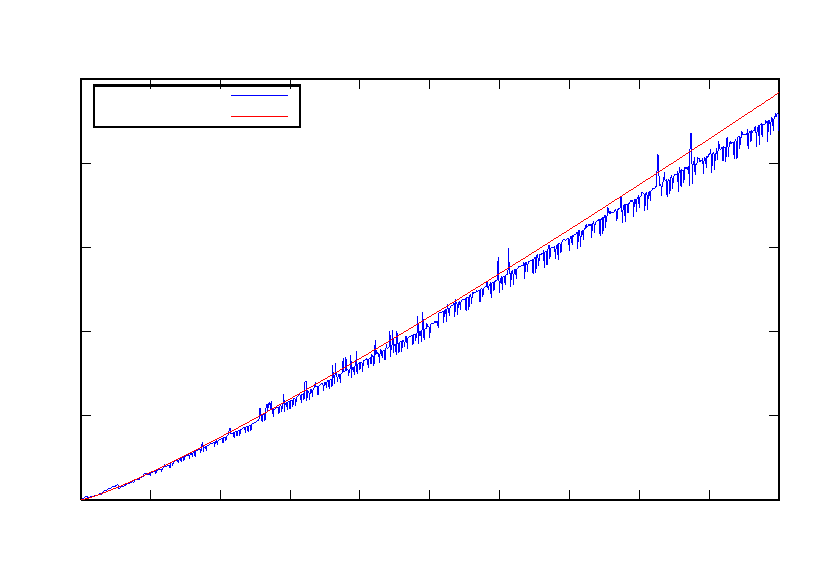
\includegraphics{problema1-peor-caso}}%
    \gplfronttext
  \end{picture}%
\endgroup

  \caption{Peor caso}
\end{figure}

\begin{figure}[H]
  \centering
  % GNUPLOT: LaTeX picture with Postscript
\begingroup
  \makeatletter
  \providecommand\color[2][]{%
    \GenericError{(gnuplot) \space\space\space\@spaces}{%
      Package color not loaded in conjunction with
      terminal option `colourtext'%
    }{See the gnuplot documentation for explanation.%
    }{Either use 'blacktext' in gnuplot or load the package
      color.sty in LaTeX.}%
    \renewcommand\color[2][]{}%
  }%
  \providecommand\includegraphics[2][]{%
    \GenericError{(gnuplot) \space\space\space\@spaces}{%
      Package graphicx or graphics not loaded%
    }{See the gnuplot documentation for explanation.%
    }{The gnuplot epslatex terminal needs graphicx.sty or graphics.sty.}%
    \renewcommand\includegraphics[2][]{}%
  }%
  \providecommand\rotatebox[2]{#2}%
  \@ifundefined{ifGPcolor}{%
    \newif\ifGPcolor
    \GPcolorfalse
  }{}%
  \@ifundefined{ifGPblacktext}{%
    \newif\ifGPblacktext
    \GPblacktexttrue
  }{}%
  % define a \g@addto@macro without @ in the name:
  \let\gplgaddtomacro\g@addto@macro
  % define empty templates for all commands taking text:
  \gdef\gplbacktext{}%
  \gdef\gplfronttext{}%
  \makeatother
  \ifGPblacktext
    % no textcolor at all
    \def\colorrgb#1{}%
    \def\colorgray#1{}%
  \else
    % gray or color?
    \ifGPcolor
      \def\colorrgb#1{\color[rgb]{#1}}%
      \def\colorgray#1{\color[gray]{#1}}%
      \expandafter\def\csname LTw\endcsname{\color{white}}%
      \expandafter\def\csname LTb\endcsname{\color{black}}%
      \expandafter\def\csname LTa\endcsname{\color{black}}%
      \expandafter\def\csname LT0\endcsname{\color[rgb]{1,0,0}}%
      \expandafter\def\csname LT1\endcsname{\color[rgb]{0,1,0}}%
      \expandafter\def\csname LT2\endcsname{\color[rgb]{0,0,1}}%
      \expandafter\def\csname LT3\endcsname{\color[rgb]{1,0,1}}%
      \expandafter\def\csname LT4\endcsname{\color[rgb]{0,1,1}}%
      \expandafter\def\csname LT5\endcsname{\color[rgb]{1,1,0}}%
      \expandafter\def\csname LT6\endcsname{\color[rgb]{0,0,0}}%
      \expandafter\def\csname LT7\endcsname{\color[rgb]{1,0.3,0}}%
      \expandafter\def\csname LT8\endcsname{\color[rgb]{0.5,0.5,0.5}}%
    \else
      % gray
      \def\colorrgb#1{\color{black}}%
      \def\colorgray#1{\color[gray]{#1}}%
      \expandafter\def\csname LTw\endcsname{\color{white}}%
      \expandafter\def\csname LTb\endcsname{\color{black}}%
      \expandafter\def\csname LTa\endcsname{\color{black}}%
      \expandafter\def\csname LT0\endcsname{\color{black}}%
      \expandafter\def\csname LT1\endcsname{\color{black}}%
      \expandafter\def\csname LT2\endcsname{\color{black}}%
      \expandafter\def\csname LT3\endcsname{\color{black}}%
      \expandafter\def\csname LT4\endcsname{\color{black}}%
      \expandafter\def\csname LT5\endcsname{\color{black}}%
      \expandafter\def\csname LT6\endcsname{\color{black}}%
      \expandafter\def\csname LT7\endcsname{\color{black}}%
      \expandafter\def\csname LT8\endcsname{\color{black}}%
    \fi
  \fi
  \setlength{\unitlength}{0.0500bp}%
  \begin{picture}(9118.00,4320.00)%
    \gplgaddtomacro\gplbacktext{%
      \colorrgb{0.00,0.00,0.00}%
      \put(500,640){\makebox(0,0)[r]{\strut{}0}}%
      \colorrgb{0.00,0.00,0.00}%
      \put(500,1153){\makebox(0,0)[r]{\strut{}1}}%
      \colorrgb{0.00,0.00,0.00}%
      \put(500,1666){\makebox(0,0)[r]{\strut{}2}}%
      \colorrgb{0.00,0.00,0.00}%
      \put(500,2180){\makebox(0,0)[r]{\strut{}3}}%
      \colorrgb{0.00,0.00,0.00}%
      \put(500,2693){\makebox(0,0)[r]{\strut{}4}}%
      \colorrgb{0.00,0.00,0.00}%
      \put(500,3206){\makebox(0,0)[r]{\strut{}5}}%
      \colorrgb{0.00,0.00,0.00}%
      \put(500,3719){\makebox(0,0)[r]{\strut{}6}}%
      \colorrgb{0.00,0.00,0.00}%
      \put(612,440){\makebox(0,0){\strut{}0}}%
      \colorrgb{0.00,0.00,0.00}%
      \put(1426,440){\makebox(0,0){\strut{}100}}%
      \colorrgb{0.00,0.00,0.00}%
      \put(2241,440){\makebox(0,0){\strut{}200}}%
      \colorrgb{0.00,0.00,0.00}%
      \put(3055,440){\makebox(0,0){\strut{}300}}%
      \colorrgb{0.00,0.00,0.00}%
      \put(3870,440){\makebox(0,0){\strut{}400}}%
      \colorrgb{0.00,0.00,0.00}%
      \put(4684,440){\makebox(0,0){\strut{}500}}%
      \colorrgb{0.00,0.00,0.00}%
      \put(5499,440){\makebox(0,0){\strut{}600}}%
      \colorrgb{0.00,0.00,0.00}%
      \put(6313,440){\makebox(0,0){\strut{}700}}%
      \colorrgb{0.00,0.00,0.00}%
      \put(7128,440){\makebox(0,0){\strut{}800}}%
      \colorrgb{0.00,0.00,0.00}%
      \put(7942,440){\makebox(0,0){\strut{}900}}%
      \colorrgb{0.00,0.00,0.00}%
      \put(8757,440){\makebox(0,0){\strut{}1000}}%
      \colorrgb{0.00,0.00,0.00}%
      \put(160,2179){\rotatebox{90}{\makebox(0,0){\strut{}Tiempo [$\mu S$]}}}%
      \colorrgb{0.00,0.00,0.00}%
      \put(4688,140){\makebox(0,0){\strut{}$n$ (tama\~no del problema)}}%
      \csname LTb\endcsname%
      \put(4688,4019){\makebox(0,0){\strut{}Tiempo de ejecuci\'on dividido por $n$}}%
    }%
    \gplgaddtomacro\gplfronttext{%
      \csname LTb\endcsname%
      \put(1820,3556){\makebox(0,0)[r]{\strut{}$T(n) / n$}}%
      \csname LTb\endcsname%
      \put(1820,3356){\makebox(0,0)[r]{\strut{}$O(log(n))$}}%
    }%
    \gplbacktext
    \put(0,0){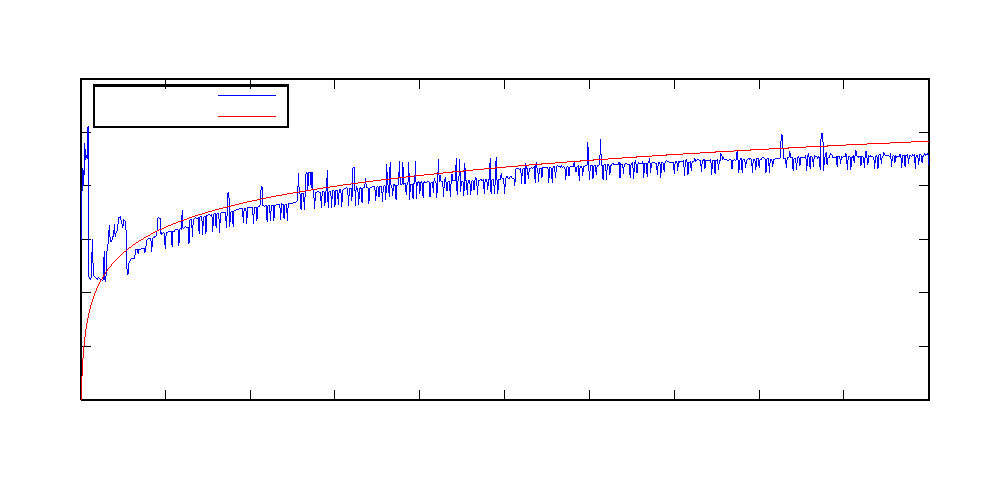
\includegraphics{problema1-peor-caso-logn}}%
    \gplfronttext
  \end{picture}%
\endgroup

  \caption{Peor caso ($log(n)$)}
\end{figure}

\begin{figure}[H]
  \centering
  % GNUPLOT: LaTeX picture with Postscript
\begingroup
  \makeatletter
  \providecommand\color[2][]{%
    \GenericError{(gnuplot) \space\space\space\@spaces}{%
      Package color not loaded in conjunction with
      terminal option `colourtext'%
    }{See the gnuplot documentation for explanation.%
    }{Either use 'blacktext' in gnuplot or load the package
      color.sty in LaTeX.}%
    \renewcommand\color[2][]{}%
  }%
  \providecommand\includegraphics[2][]{%
    \GenericError{(gnuplot) \space\space\space\@spaces}{%
      Package graphicx or graphics not loaded%
    }{See the gnuplot documentation for explanation.%
    }{The gnuplot epslatex terminal needs graphicx.sty or graphics.sty.}%
    \renewcommand\includegraphics[2][]{}%
  }%
  \providecommand\rotatebox[2]{#2}%
  \@ifundefined{ifGPcolor}{%
    \newif\ifGPcolor
    \GPcolorfalse
  }{}%
  \@ifundefined{ifGPblacktext}{%
    \newif\ifGPblacktext
    \GPblacktexttrue
  }{}%
  % define a \g@addto@macro without @ in the name:
  \let\gplgaddtomacro\g@addto@macro
  % define empty templates for all commands taking text:
  \gdef\gplbacktext{}%
  \gdef\gplfronttext{}%
  \makeatother
  \ifGPblacktext
    % no textcolor at all
    \def\colorrgb#1{}%
    \def\colorgray#1{}%
  \else
    % gray or color?
    \ifGPcolor
      \def\colorrgb#1{\color[rgb]{#1}}%
      \def\colorgray#1{\color[gray]{#1}}%
      \expandafter\def\csname LTw\endcsname{\color{white}}%
      \expandafter\def\csname LTb\endcsname{\color{black}}%
      \expandafter\def\csname LTa\endcsname{\color{black}}%
      \expandafter\def\csname LT0\endcsname{\color[rgb]{1,0,0}}%
      \expandafter\def\csname LT1\endcsname{\color[rgb]{0,1,0}}%
      \expandafter\def\csname LT2\endcsname{\color[rgb]{0,0,1}}%
      \expandafter\def\csname LT3\endcsname{\color[rgb]{1,0,1}}%
      \expandafter\def\csname LT4\endcsname{\color[rgb]{0,1,1}}%
      \expandafter\def\csname LT5\endcsname{\color[rgb]{1,1,0}}%
      \expandafter\def\csname LT6\endcsname{\color[rgb]{0,0,0}}%
      \expandafter\def\csname LT7\endcsname{\color[rgb]{1,0.3,0}}%
      \expandafter\def\csname LT8\endcsname{\color[rgb]{0.5,0.5,0.5}}%
    \else
      % gray
      \def\colorrgb#1{\color{black}}%
      \def\colorgray#1{\color[gray]{#1}}%
      \expandafter\def\csname LTw\endcsname{\color{white}}%
      \expandafter\def\csname LTb\endcsname{\color{black}}%
      \expandafter\def\csname LTa\endcsname{\color{black}}%
      \expandafter\def\csname LT0\endcsname{\color{black}}%
      \expandafter\def\csname LT1\endcsname{\color{black}}%
      \expandafter\def\csname LT2\endcsname{\color{black}}%
      \expandafter\def\csname LT3\endcsname{\color{black}}%
      \expandafter\def\csname LT4\endcsname{\color{black}}%
      \expandafter\def\csname LT5\endcsname{\color{black}}%
      \expandafter\def\csname LT6\endcsname{\color{black}}%
      \expandafter\def\csname LT7\endcsname{\color{black}}%
      \expandafter\def\csname LT8\endcsname{\color{black}}%
    \fi
  \fi
  \setlength{\unitlength}{0.0500bp}%
  \begin{picture}(9118.00,4320.00)%
    \gplgaddtomacro\gplbacktext{%
      \colorrgb{0.00,0.00,0.00}%
      \put(740,640){\makebox(0,0)[r]{\strut{}0}}%
      \colorrgb{0.00,0.00,0.00}%
      \put(740,1080){\makebox(0,0)[r]{\strut{}0.1}}%
      \colorrgb{0.00,0.00,0.00}%
      \put(740,1520){\makebox(0,0)[r]{\strut{}0.2}}%
      \colorrgb{0.00,0.00,0.00}%
      \put(740,1960){\makebox(0,0)[r]{\strut{}0.3}}%
      \colorrgb{0.00,0.00,0.00}%
      \put(740,2399){\makebox(0,0)[r]{\strut{}0.4}}%
      \colorrgb{0.00,0.00,0.00}%
      \put(740,2839){\makebox(0,0)[r]{\strut{}0.5}}%
      \colorrgb{0.00,0.00,0.00}%
      \put(740,3279){\makebox(0,0)[r]{\strut{}0.6}}%
      \colorrgb{0.00,0.00,0.00}%
      \put(740,3719){\makebox(0,0)[r]{\strut{}0.7}}%
      \colorrgb{0.00,0.00,0.00}%
      \put(852,440){\makebox(0,0){\strut{}0}}%
      \colorrgb{0.00,0.00,0.00}%
      \put(1643,440){\makebox(0,0){\strut{}100}}%
      \colorrgb{0.00,0.00,0.00}%
      \put(2433,440){\makebox(0,0){\strut{}200}}%
      \colorrgb{0.00,0.00,0.00}%
      \put(3224,440){\makebox(0,0){\strut{}300}}%
      \colorrgb{0.00,0.00,0.00}%
      \put(4014,440){\makebox(0,0){\strut{}400}}%
      \colorrgb{0.00,0.00,0.00}%
      \put(4805,440){\makebox(0,0){\strut{}500}}%
      \colorrgb{0.00,0.00,0.00}%
      \put(5595,440){\makebox(0,0){\strut{}600}}%
      \colorrgb{0.00,0.00,0.00}%
      \put(6386,440){\makebox(0,0){\strut{}700}}%
      \colorrgb{0.00,0.00,0.00}%
      \put(7176,440){\makebox(0,0){\strut{}800}}%
      \colorrgb{0.00,0.00,0.00}%
      \put(7967,440){\makebox(0,0){\strut{}900}}%
      \colorrgb{0.00,0.00,0.00}%
      \put(8757,440){\makebox(0,0){\strut{}1000}}%
      \colorrgb{0.00,0.00,0.00}%
      \put(160,2179){\rotatebox{90}{\makebox(0,0){\strut{}Tiempo [$mS$]}}}%
      \colorrgb{0.00,0.00,0.00}%
      \put(4808,140){\makebox(0,0){\strut{}$n$ (tama\~no del problema)}}%
      \csname LTb\endcsname%
      \put(4808,4019){\makebox(0,0){\strut{}Tiempo de ejecuci\'on dividido por $log(n)$}}%
    }%
    \gplgaddtomacro\gplfronttext{%
      \csname LTb\endcsname%
      \put(2540,3556){\makebox(0,0)[r]{\strut{}$T(n) / log(n)$}}%
      \csname LTb\endcsname%
      \put(2540,3356){\makebox(0,0)[r]{\strut{}$O(n)$}}%
    }%
    \gplbacktext
    \put(0,0){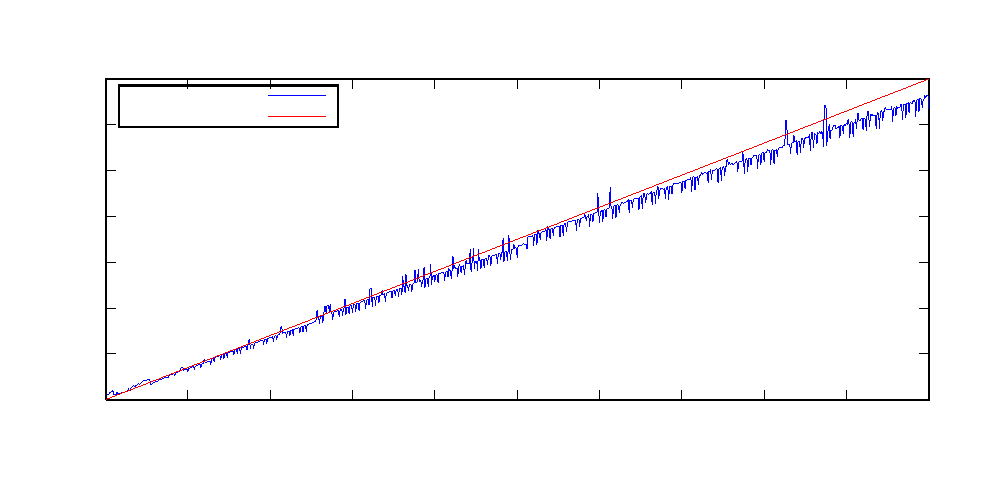
\includegraphics{problema1-peor-caso-n}}%
    \gplfronttext
  \end{picture}%
\endgroup

  \caption{Peor caso ($n$)}
\end{figure}


\subsubsection{Mejor caso}

\begin{figure}[H]
  \centering
  % GNUPLOT: LaTeX picture with Postscript
\begingroup
  \makeatletter
  \providecommand\color[2][]{%
    \GenericError{(gnuplot) \space\space\space\@spaces}{%
      Package color not loaded in conjunction with
      terminal option `colourtext'%
    }{See the gnuplot documentation for explanation.%
    }{Either use 'blacktext' in gnuplot or load the package
      color.sty in LaTeX.}%
    \renewcommand\color[2][]{}%
  }%
  \providecommand\includegraphics[2][]{%
    \GenericError{(gnuplot) \space\space\space\@spaces}{%
      Package graphicx or graphics not loaded%
    }{See the gnuplot documentation for explanation.%
    }{The gnuplot epslatex terminal needs graphicx.sty or graphics.sty.}%
    \renewcommand\includegraphics[2][]{}%
  }%
  \providecommand\rotatebox[2]{#2}%
  \@ifundefined{ifGPcolor}{%
    \newif\ifGPcolor
    \GPcolorfalse
  }{}%
  \@ifundefined{ifGPblacktext}{%
    \newif\ifGPblacktext
    \GPblacktexttrue
  }{}%
  % define a \g@addto@macro without @ in the name:
  \let\gplgaddtomacro\g@addto@macro
  % define empty templates for all commands taking text:
  \gdef\gplbacktext{}%
  \gdef\gplfronttext{}%
  \makeatother
  \ifGPblacktext
    % no textcolor at all
    \def\colorrgb#1{}%
    \def\colorgray#1{}%
  \else
    % gray or color?
    \ifGPcolor
      \def\colorrgb#1{\color[rgb]{#1}}%
      \def\colorgray#1{\color[gray]{#1}}%
      \expandafter\def\csname LTw\endcsname{\color{white}}%
      \expandafter\def\csname LTb\endcsname{\color{black}}%
      \expandafter\def\csname LTa\endcsname{\color{black}}%
      \expandafter\def\csname LT0\endcsname{\color[rgb]{1,0,0}}%
      \expandafter\def\csname LT1\endcsname{\color[rgb]{0,1,0}}%
      \expandafter\def\csname LT2\endcsname{\color[rgb]{0,0,1}}%
      \expandafter\def\csname LT3\endcsname{\color[rgb]{1,0,1}}%
      \expandafter\def\csname LT4\endcsname{\color[rgb]{0,1,1}}%
      \expandafter\def\csname LT5\endcsname{\color[rgb]{1,1,0}}%
      \expandafter\def\csname LT6\endcsname{\color[rgb]{0,0,0}}%
      \expandafter\def\csname LT7\endcsname{\color[rgb]{1,0.3,0}}%
      \expandafter\def\csname LT8\endcsname{\color[rgb]{0.5,0.5,0.5}}%
    \else
      % gray
      \def\colorrgb#1{\color{black}}%
      \def\colorgray#1{\color[gray]{#1}}%
      \expandafter\def\csname LTw\endcsname{\color{white}}%
      \expandafter\def\csname LTb\endcsname{\color{black}}%
      \expandafter\def\csname LTa\endcsname{\color{black}}%
      \expandafter\def\csname LT0\endcsname{\color{black}}%
      \expandafter\def\csname LT1\endcsname{\color{black}}%
      \expandafter\def\csname LT2\endcsname{\color{black}}%
      \expandafter\def\csname LT3\endcsname{\color{black}}%
      \expandafter\def\csname LT4\endcsname{\color{black}}%
      \expandafter\def\csname LT5\endcsname{\color{black}}%
      \expandafter\def\csname LT6\endcsname{\color{black}}%
      \expandafter\def\csname LT7\endcsname{\color{black}}%
      \expandafter\def\csname LT8\endcsname{\color{black}}%
    \fi
  \fi
  \setlength{\unitlength}{0.0500bp}%
  \begin{picture}(7678.00,5280.00)%
    \gplgaddtomacro\gplbacktext{%
      \colorrgb{0.00,0.00,0.00}%
      \put(740,640){\makebox(0,0)[r]{\strut{}0}}%
      \colorrgb{0.00,0.00,0.00}%
      \put(740,1448){\makebox(0,0)[r]{\strut{}0.1}}%
      \colorrgb{0.00,0.00,0.00}%
      \put(740,2256){\makebox(0,0)[r]{\strut{}0.2}}%
      \colorrgb{0.00,0.00,0.00}%
      \put(740,3063){\makebox(0,0)[r]{\strut{}0.3}}%
      \colorrgb{0.00,0.00,0.00}%
      \put(740,3871){\makebox(0,0)[r]{\strut{}0.4}}%
      \colorrgb{0.00,0.00,0.00}%
      \put(740,4679){\makebox(0,0)[r]{\strut{}0.5}}%
      \colorrgb{0.00,0.00,0.00}%
      \put(854,440){\makebox(0,0){\strut{}0}}%
      \colorrgb{0.00,0.00,0.00}%
      \put(1500,440){\makebox(0,0){\strut{}100}}%
      \colorrgb{0.00,0.00,0.00}%
      \put(2146,440){\makebox(0,0){\strut{}200}}%
      \colorrgb{0.00,0.00,0.00}%
      \put(2793,440){\makebox(0,0){\strut{}300}}%
      \colorrgb{0.00,0.00,0.00}%
      \put(3439,440){\makebox(0,0){\strut{}400}}%
      \colorrgb{0.00,0.00,0.00}%
      \put(4085,440){\makebox(0,0){\strut{}500}}%
      \colorrgb{0.00,0.00,0.00}%
      \put(4732,440){\makebox(0,0){\strut{}600}}%
      \colorrgb{0.00,0.00,0.00}%
      \put(5378,440){\makebox(0,0){\strut{}700}}%
      \colorrgb{0.00,0.00,0.00}%
      \put(6024,440){\makebox(0,0){\strut{}800}}%
      \colorrgb{0.00,0.00,0.00}%
      \put(6671,440){\makebox(0,0){\strut{}900}}%
      \colorrgb{0.00,0.00,0.00}%
      \put(7317,440){\makebox(0,0){\strut{}1000}}%
      \colorrgb{0.00,0.00,0.00}%
      \put(160,2659){\rotatebox{90}{\makebox(0,0){\strut{}Tiempo de ejecución [$mS$]}}}%
      \colorrgb{0.00,0.00,0.00}%
      \put(4088,140){\makebox(0,0){\strut{}$n$ (tamaño del problema)}}%
      \csname LTb\endcsname%
      \put(4088,4979){\makebox(0,0){\strut{}Mejor caso}}%
    }%
    \gplgaddtomacro\gplfronttext{%
      \csname LTb\endcsname%
      \put(2180,4516){\makebox(0,0)[r]{\strut{}$t_n$}}%
      \csname LTb\endcsname%
      \put(2180,4316){\makebox(0,0)[r]{\strut{}$n * log(n)$}}%
    }%
    \gplbacktext
    \put(0,0){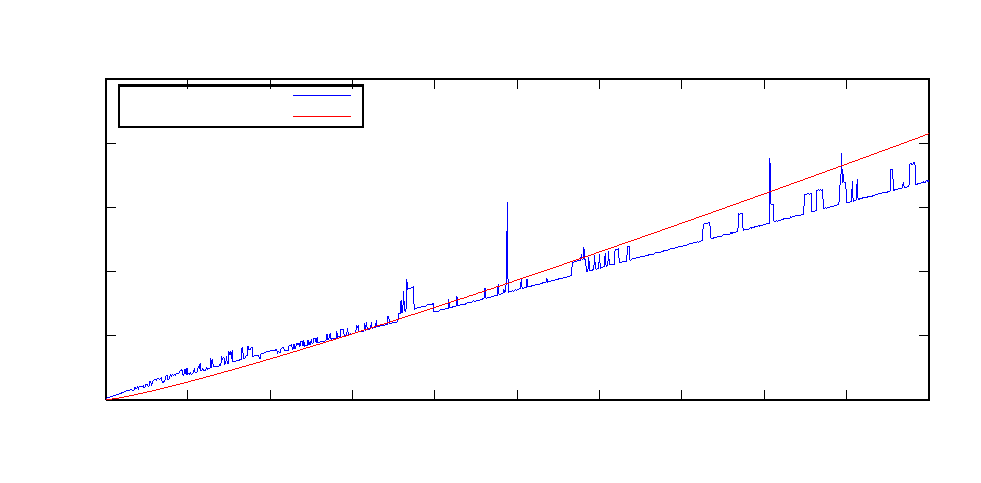
\includegraphics{problema1-mejor-caso}}%
    \gplfronttext
  \end{picture}%
\endgroup

  \caption{Mejor caso}
\end{figure}

\begin{figure}[H]
  \centering
  % GNUPLOT: LaTeX picture with Postscript
\begingroup
  \makeatletter
  \providecommand\color[2][]{%
    \GenericError{(gnuplot) \space\space\space\@spaces}{%
      Package color not loaded in conjunction with
      terminal option `colourtext'%
    }{See the gnuplot documentation for explanation.%
    }{Either use 'blacktext' in gnuplot or load the package
      color.sty in LaTeX.}%
    \renewcommand\color[2][]{}%
  }%
  \providecommand\includegraphics[2][]{%
    \GenericError{(gnuplot) \space\space\space\@spaces}{%
      Package graphicx or graphics not loaded%
    }{See the gnuplot documentation for explanation.%
    }{The gnuplot epslatex terminal needs graphicx.sty or graphics.sty.}%
    \renewcommand\includegraphics[2][]{}%
  }%
  \providecommand\rotatebox[2]{#2}%
  \@ifundefined{ifGPcolor}{%
    \newif\ifGPcolor
    \GPcolorfalse
  }{}%
  \@ifundefined{ifGPblacktext}{%
    \newif\ifGPblacktext
    \GPblacktexttrue
  }{}%
  % define a \g@addto@macro without @ in the name:
  \let\gplgaddtomacro\g@addto@macro
  % define empty templates for all commands taking text:
  \gdef\gplbacktext{}%
  \gdef\gplfronttext{}%
  \makeatother
  \ifGPblacktext
    % no textcolor at all
    \def\colorrgb#1{}%
    \def\colorgray#1{}%
  \else
    % gray or color?
    \ifGPcolor
      \def\colorrgb#1{\color[rgb]{#1}}%
      \def\colorgray#1{\color[gray]{#1}}%
      \expandafter\def\csname LTw\endcsname{\color{white}}%
      \expandafter\def\csname LTb\endcsname{\color{black}}%
      \expandafter\def\csname LTa\endcsname{\color{black}}%
      \expandafter\def\csname LT0\endcsname{\color[rgb]{1,0,0}}%
      \expandafter\def\csname LT1\endcsname{\color[rgb]{0,1,0}}%
      \expandafter\def\csname LT2\endcsname{\color[rgb]{0,0,1}}%
      \expandafter\def\csname LT3\endcsname{\color[rgb]{1,0,1}}%
      \expandafter\def\csname LT4\endcsname{\color[rgb]{0,1,1}}%
      \expandafter\def\csname LT5\endcsname{\color[rgb]{1,1,0}}%
      \expandafter\def\csname LT6\endcsname{\color[rgb]{0,0,0}}%
      \expandafter\def\csname LT7\endcsname{\color[rgb]{1,0.3,0}}%
      \expandafter\def\csname LT8\endcsname{\color[rgb]{0.5,0.5,0.5}}%
    \else
      % gray
      \def\colorrgb#1{\color{black}}%
      \def\colorgray#1{\color[gray]{#1}}%
      \expandafter\def\csname LTw\endcsname{\color{white}}%
      \expandafter\def\csname LTb\endcsname{\color{black}}%
      \expandafter\def\csname LTa\endcsname{\color{black}}%
      \expandafter\def\csname LT0\endcsname{\color{black}}%
      \expandafter\def\csname LT1\endcsname{\color{black}}%
      \expandafter\def\csname LT2\endcsname{\color{black}}%
      \expandafter\def\csname LT3\endcsname{\color{black}}%
      \expandafter\def\csname LT4\endcsname{\color{black}}%
      \expandafter\def\csname LT5\endcsname{\color{black}}%
      \expandafter\def\csname LT6\endcsname{\color{black}}%
      \expandafter\def\csname LT7\endcsname{\color{black}}%
      \expandafter\def\csname LT8\endcsname{\color{black}}%
    \fi
  \fi
  \setlength{\unitlength}{0.0500bp}%
  \begin{picture}(7678.00,5280.00)%
    \gplgaddtomacro\gplbacktext{%
      \colorrgb{0.00,0.00,0.00}%
      \put(1100,640){\makebox(0,0)[r]{\strut{}0}}%
      \colorrgb{0.00,0.00,0.00}%
      \put(1100,1650){\makebox(0,0)[r]{\strut{}0.0005}}%
      \colorrgb{0.00,0.00,0.00}%
      \put(1100,2660){\makebox(0,0)[r]{\strut{}0.001}}%
      \colorrgb{0.00,0.00,0.00}%
      \put(1100,3669){\makebox(0,0)[r]{\strut{}0.0015}}%
      \colorrgb{0.00,0.00,0.00}%
      \put(1100,4679){\makebox(0,0)[r]{\strut{}0.002}}%
      \colorrgb{0.00,0.00,0.00}%
      \put(1214,440){\makebox(0,0){\strut{}0}}%
      \colorrgb{0.00,0.00,0.00}%
      \put(1824,440){\makebox(0,0){\strut{}100}}%
      \colorrgb{0.00,0.00,0.00}%
      \put(2435,440){\makebox(0,0){\strut{}200}}%
      \colorrgb{0.00,0.00,0.00}%
      \put(3045,440){\makebox(0,0){\strut{}300}}%
      \colorrgb{0.00,0.00,0.00}%
      \put(3655,440){\makebox(0,0){\strut{}400}}%
      \colorrgb{0.00,0.00,0.00}%
      \put(4265,440){\makebox(0,0){\strut{}500}}%
      \colorrgb{0.00,0.00,0.00}%
      \put(4876,440){\makebox(0,0){\strut{}600}}%
      \colorrgb{0.00,0.00,0.00}%
      \put(5486,440){\makebox(0,0){\strut{}700}}%
      \colorrgb{0.00,0.00,0.00}%
      \put(6096,440){\makebox(0,0){\strut{}800}}%
      \colorrgb{0.00,0.00,0.00}%
      \put(6707,440){\makebox(0,0){\strut{}900}}%
      \colorrgb{0.00,0.00,0.00}%
      \put(7317,440){\makebox(0,0){\strut{}1000}}%
      \colorrgb{0.00,0.00,0.00}%
      \put(160,2659){\rotatebox{90}{\makebox(0,0){\strut{}Tiempo de ejecuci\'on [$mS$]}}}%
      \colorrgb{0.00,0.00,0.00}%
      \put(4268,140){\makebox(0,0){\strut{}$n$ (tama\~no del problema)}}%
      \csname LTb\endcsname%
      \put(4268,4979){\makebox(0,0){\strut{}Mejor caso ($log(n)$)}}%
    }%
    \gplgaddtomacro\gplfronttext{%
      \csname LTb\endcsname%
      \put(2060,4516){\makebox(0,0)[r]{\strut{}$t_n / n$}}%
      \csname LTb\endcsname%
      \put(2060,4316){\makebox(0,0)[r]{\strut{}$log(n)$}}%
    }%
    \gplbacktext
    \put(0,0){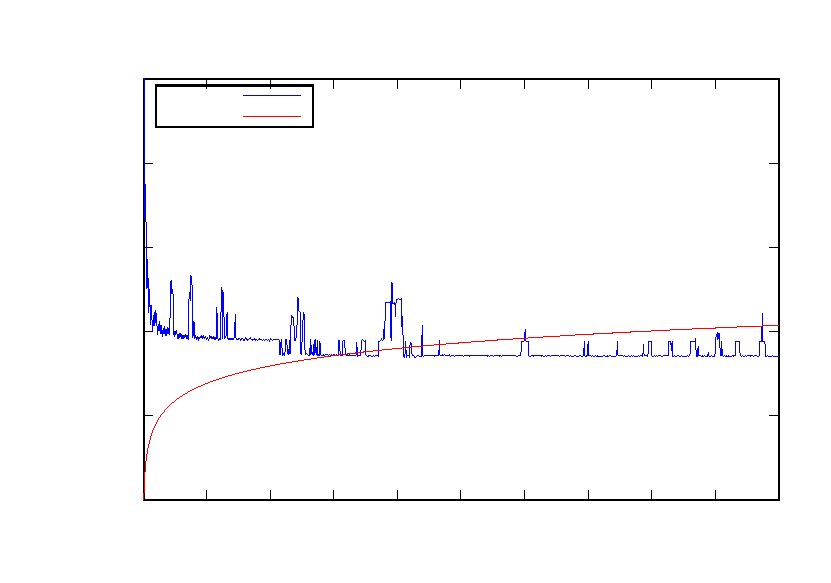
\includegraphics{problema1-mejor-caso-logn}}%
    \gplfronttext
  \end{picture}%
\endgroup

  \caption{Mejor caso ($log(n)$)}
\end{figure}

\begin{figure}[H]
  \centering
  % GNUPLOT: LaTeX picture with Postscript
\begingroup
  \makeatletter
  \providecommand\color[2][]{%
    \GenericError{(gnuplot) \space\space\space\@spaces}{%
      Package color not loaded in conjunction with
      terminal option `colourtext'%
    }{See the gnuplot documentation for explanation.%
    }{Either use 'blacktext' in gnuplot or load the package
      color.sty in LaTeX.}%
    \renewcommand\color[2][]{}%
  }%
  \providecommand\includegraphics[2][]{%
    \GenericError{(gnuplot) \space\space\space\@spaces}{%
      Package graphicx or graphics not loaded%
    }{See the gnuplot documentation for explanation.%
    }{The gnuplot epslatex terminal needs graphicx.sty or graphics.sty.}%
    \renewcommand\includegraphics[2][]{}%
  }%
  \providecommand\rotatebox[2]{#2}%
  \@ifundefined{ifGPcolor}{%
    \newif\ifGPcolor
    \GPcolorfalse
  }{}%
  \@ifundefined{ifGPblacktext}{%
    \newif\ifGPblacktext
    \GPblacktexttrue
  }{}%
  % define a \g@addto@macro without @ in the name:
  \let\gplgaddtomacro\g@addto@macro
  % define empty templates for all commands taking text:
  \gdef\gplbacktext{}%
  \gdef\gplfronttext{}%
  \makeatother
  \ifGPblacktext
    % no textcolor at all
    \def\colorrgb#1{}%
    \def\colorgray#1{}%
  \else
    % gray or color?
    \ifGPcolor
      \def\colorrgb#1{\color[rgb]{#1}}%
      \def\colorgray#1{\color[gray]{#1}}%
      \expandafter\def\csname LTw\endcsname{\color{white}}%
      \expandafter\def\csname LTb\endcsname{\color{black}}%
      \expandafter\def\csname LTa\endcsname{\color{black}}%
      \expandafter\def\csname LT0\endcsname{\color[rgb]{1,0,0}}%
      \expandafter\def\csname LT1\endcsname{\color[rgb]{0,1,0}}%
      \expandafter\def\csname LT2\endcsname{\color[rgb]{0,0,1}}%
      \expandafter\def\csname LT3\endcsname{\color[rgb]{1,0,1}}%
      \expandafter\def\csname LT4\endcsname{\color[rgb]{0,1,1}}%
      \expandafter\def\csname LT5\endcsname{\color[rgb]{1,1,0}}%
      \expandafter\def\csname LT6\endcsname{\color[rgb]{0,0,0}}%
      \expandafter\def\csname LT7\endcsname{\color[rgb]{1,0.3,0}}%
      \expandafter\def\csname LT8\endcsname{\color[rgb]{0.5,0.5,0.5}}%
    \else
      % gray
      \def\colorrgb#1{\color{black}}%
      \def\colorgray#1{\color[gray]{#1}}%
      \expandafter\def\csname LTw\endcsname{\color{white}}%
      \expandafter\def\csname LTb\endcsname{\color{black}}%
      \expandafter\def\csname LTa\endcsname{\color{black}}%
      \expandafter\def\csname LT0\endcsname{\color{black}}%
      \expandafter\def\csname LT1\endcsname{\color{black}}%
      \expandafter\def\csname LT2\endcsname{\color{black}}%
      \expandafter\def\csname LT3\endcsname{\color{black}}%
      \expandafter\def\csname LT4\endcsname{\color{black}}%
      \expandafter\def\csname LT5\endcsname{\color{black}}%
      \expandafter\def\csname LT6\endcsname{\color{black}}%
      \expandafter\def\csname LT7\endcsname{\color{black}}%
      \expandafter\def\csname LT8\endcsname{\color{black}}%
    \fi
  \fi
  \setlength{\unitlength}{0.0500bp}%
  \begin{picture}(9118.00,4320.00)%
    \gplgaddtomacro\gplbacktext{%
      \colorrgb{0.00,0.00,0.00}%
      \put(860,640){\makebox(0,0)[r]{\strut{}0}}%
      \colorrgb{0.00,0.00,0.00}%
      \put(860,1153){\makebox(0,0)[r]{\strut{}0.01}}%
      \colorrgb{0.00,0.00,0.00}%
      \put(860,1666){\makebox(0,0)[r]{\strut{}0.02}}%
      \colorrgb{0.00,0.00,0.00}%
      \put(860,2180){\makebox(0,0)[r]{\strut{}0.03}}%
      \colorrgb{0.00,0.00,0.00}%
      \put(860,2693){\makebox(0,0)[r]{\strut{}0.04}}%
      \colorrgb{0.00,0.00,0.00}%
      \put(860,3206){\makebox(0,0)[r]{\strut{}0.05}}%
      \colorrgb{0.00,0.00,0.00}%
      \put(860,3719){\makebox(0,0)[r]{\strut{}0.06}}%
      \colorrgb{0.00,0.00,0.00}%
      \put(972,440){\makebox(0,0){\strut{}0}}%
      \colorrgb{0.00,0.00,0.00}%
      \put(1751,440){\makebox(0,0){\strut{}100}}%
      \colorrgb{0.00,0.00,0.00}%
      \put(2529,440){\makebox(0,0){\strut{}200}}%
      \colorrgb{0.00,0.00,0.00}%
      \put(3308,440){\makebox(0,0){\strut{}300}}%
      \colorrgb{0.00,0.00,0.00}%
      \put(4086,440){\makebox(0,0){\strut{}400}}%
      \colorrgb{0.00,0.00,0.00}%
      \put(4865,440){\makebox(0,0){\strut{}500}}%
      \colorrgb{0.00,0.00,0.00}%
      \put(5643,440){\makebox(0,0){\strut{}600}}%
      \colorrgb{0.00,0.00,0.00}%
      \put(6422,440){\makebox(0,0){\strut{}700}}%
      \colorrgb{0.00,0.00,0.00}%
      \put(7200,440){\makebox(0,0){\strut{}800}}%
      \colorrgb{0.00,0.00,0.00}%
      \put(7979,440){\makebox(0,0){\strut{}900}}%
      \colorrgb{0.00,0.00,0.00}%
      \put(8757,440){\makebox(0,0){\strut{}1000}}%
      \colorrgb{0.00,0.00,0.00}%
      \put(160,2179){\rotatebox{90}{\makebox(0,0){\strut{}Tiempo [$mS$]}}}%
      \colorrgb{0.00,0.00,0.00}%
      \put(4868,140){\makebox(0,0){\strut{}$n$ (tama\~no del problema)}}%
      \csname LTb\endcsname%
      \put(4868,4019){\makebox(0,0){\strut{}Tiempo de ejecuci\'on dividido por $log(n)$}}%
    }%
    \gplgaddtomacro\gplfronttext{%
      \csname LTb\endcsname%
      \put(2660,3556){\makebox(0,0)[r]{\strut{}$T(n) / log(n)$}}%
      \csname LTb\endcsname%
      \put(2660,3356){\makebox(0,0)[r]{\strut{}$O(n)$}}%
    }%
    \gplbacktext
    \put(0,0){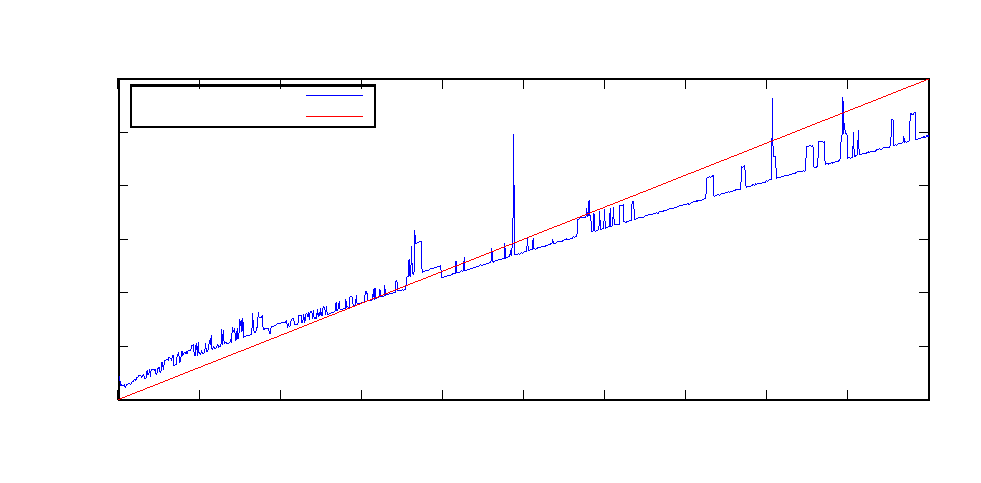
\includegraphics{problema1-mejor-caso-n}}%
    \gplfronttext
  \end{picture}%
\endgroup

  \caption{Mejor caso ($n$)}
\end{figure}


\subsubsection{Instancias aleatorias}

\begin{figure}[H]
  \centering
  % GNUPLOT: LaTeX picture with Postscript
\begingroup
  \makeatletter
  \providecommand\color[2][]{%
    \GenericError{(gnuplot) \space\space\space\@spaces}{%
      Package color not loaded in conjunction with
      terminal option `colourtext'%
    }{See the gnuplot documentation for explanation.%
    }{Either use 'blacktext' in gnuplot or load the package
      color.sty in LaTeX.}%
    \renewcommand\color[2][]{}%
  }%
  \providecommand\includegraphics[2][]{%
    \GenericError{(gnuplot) \space\space\space\@spaces}{%
      Package graphicx or graphics not loaded%
    }{See the gnuplot documentation for explanation.%
    }{The gnuplot epslatex terminal needs graphicx.sty or graphics.sty.}%
    \renewcommand\includegraphics[2][]{}%
  }%
  \providecommand\rotatebox[2]{#2}%
  \@ifundefined{ifGPcolor}{%
    \newif\ifGPcolor
    \GPcolorfalse
  }{}%
  \@ifundefined{ifGPblacktext}{%
    \newif\ifGPblacktext
    \GPblacktexttrue
  }{}%
  % define a \g@addto@macro without @ in the name:
  \let\gplgaddtomacro\g@addto@macro
  % define empty templates for all commands taking text:
  \gdef\gplbacktext{}%
  \gdef\gplfronttext{}%
  \makeatother
  \ifGPblacktext
    % no textcolor at all
    \def\colorrgb#1{}%
    \def\colorgray#1{}%
  \else
    % gray or color?
    \ifGPcolor
      \def\colorrgb#1{\color[rgb]{#1}}%
      \def\colorgray#1{\color[gray]{#1}}%
      \expandafter\def\csname LTw\endcsname{\color{white}}%
      \expandafter\def\csname LTb\endcsname{\color{black}}%
      \expandafter\def\csname LTa\endcsname{\color{black}}%
      \expandafter\def\csname LT0\endcsname{\color[rgb]{1,0,0}}%
      \expandafter\def\csname LT1\endcsname{\color[rgb]{0,1,0}}%
      \expandafter\def\csname LT2\endcsname{\color[rgb]{0,0,1}}%
      \expandafter\def\csname LT3\endcsname{\color[rgb]{1,0,1}}%
      \expandafter\def\csname LT4\endcsname{\color[rgb]{0,1,1}}%
      \expandafter\def\csname LT5\endcsname{\color[rgb]{1,1,0}}%
      \expandafter\def\csname LT6\endcsname{\color[rgb]{0,0,0}}%
      \expandafter\def\csname LT7\endcsname{\color[rgb]{1,0.3,0}}%
      \expandafter\def\csname LT8\endcsname{\color[rgb]{0.5,0.5,0.5}}%
    \else
      % gray
      \def\colorrgb#1{\color{black}}%
      \def\colorgray#1{\color[gray]{#1}}%
      \expandafter\def\csname LTw\endcsname{\color{white}}%
      \expandafter\def\csname LTb\endcsname{\color{black}}%
      \expandafter\def\csname LTa\endcsname{\color{black}}%
      \expandafter\def\csname LT0\endcsname{\color{black}}%
      \expandafter\def\csname LT1\endcsname{\color{black}}%
      \expandafter\def\csname LT2\endcsname{\color{black}}%
      \expandafter\def\csname LT3\endcsname{\color{black}}%
      \expandafter\def\csname LT4\endcsname{\color{black}}%
      \expandafter\def\csname LT5\endcsname{\color{black}}%
      \expandafter\def\csname LT6\endcsname{\color{black}}%
      \expandafter\def\csname LT7\endcsname{\color{black}}%
      \expandafter\def\csname LT8\endcsname{\color{black}}%
    \fi
  \fi
  \setlength{\unitlength}{0.0500bp}%
  \begin{picture}(7678.00,5280.00)%
    \gplgaddtomacro\gplbacktext{%
      \colorrgb{0.00,0.00,0.00}%
      \put(500,640){\makebox(0,0)[r]{\strut{}0}}%
      \colorrgb{0.00,0.00,0.00}%
      \put(500,1448){\makebox(0,0)[r]{\strut{}1}}%
      \colorrgb{0.00,0.00,0.00}%
      \put(500,2256){\makebox(0,0)[r]{\strut{}2}}%
      \colorrgb{0.00,0.00,0.00}%
      \put(500,3063){\makebox(0,0)[r]{\strut{}3}}%
      \colorrgb{0.00,0.00,0.00}%
      \put(500,3871){\makebox(0,0)[r]{\strut{}4}}%
      \colorrgb{0.00,0.00,0.00}%
      \put(500,4679){\makebox(0,0)[r]{\strut{}5}}%
      \colorrgb{0.00,0.00,0.00}%
      \put(620,440){\makebox(0,0){\strut{}100}}%
      \colorrgb{0.00,0.00,0.00}%
      \put(1456,440){\makebox(0,0){\strut{}200}}%
      \colorrgb{0.00,0.00,0.00}%
      \put(2292,440){\makebox(0,0){\strut{}300}}%
      \colorrgb{0.00,0.00,0.00}%
      \put(3128,440){\makebox(0,0){\strut{}400}}%
      \colorrgb{0.00,0.00,0.00}%
      \put(3964,440){\makebox(0,0){\strut{}500}}%
      \colorrgb{0.00,0.00,0.00}%
      \put(4800,440){\makebox(0,0){\strut{}600}}%
      \colorrgb{0.00,0.00,0.00}%
      \put(5636,440){\makebox(0,0){\strut{}700}}%
      \colorrgb{0.00,0.00,0.00}%
      \put(6473,440){\makebox(0,0){\strut{}800}}%
      \colorrgb{0.00,0.00,0.00}%
      \put(7309,440){\makebox(0,0){\strut{}900}}%
      \colorrgb{0.00,0.00,0.00}%
      \put(160,2659){\rotatebox{90}{\makebox(0,0){\strut{}Tiempo de ejecuci\'on [$mS$]}}}%
      \colorrgb{0.00,0.00,0.00}%
      \put(3968,140){\makebox(0,0){\strut{}$n$ (tama\~no del problema)}}%
      \csname LTb\endcsname%
      \put(3968,4979){\makebox(0,0){\strut{}Instancias aleatorias}}%
    }%
    \gplgaddtomacro\gplfronttext{%
      \csname LTb\endcsname%
      \put(1940,4516){\makebox(0,0)[r]{\strut{}$t_n$}}%
      \csname LTb\endcsname%
      \put(1940,4316){\makebox(0,0)[r]{\strut{}$n * log(n)$}}%
    }%
    \gplbacktext
    \put(0,0){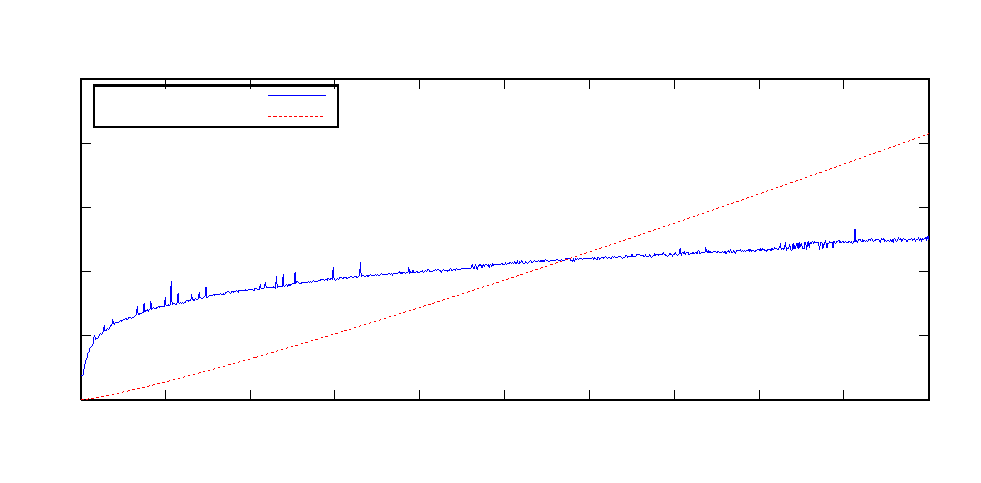
\includegraphics{problema1-instancias-aleatorias}}%
    \gplfronttext
  \end{picture}%
\endgroup

  \caption{Instancias aleatorias}
\end{figure}

\begin{figure}[H]
  \centering
  % GNUPLOT: LaTeX picture with Postscript
\begingroup
  \makeatletter
  \providecommand\color[2][]{%
    \GenericError{(gnuplot) \space\space\space\@spaces}{%
      Package color not loaded in conjunction with
      terminal option `colourtext'%
    }{See the gnuplot documentation for explanation.%
    }{Either use 'blacktext' in gnuplot or load the package
      color.sty in LaTeX.}%
    \renewcommand\color[2][]{}%
  }%
  \providecommand\includegraphics[2][]{%
    \GenericError{(gnuplot) \space\space\space\@spaces}{%
      Package graphicx or graphics not loaded%
    }{See the gnuplot documentation for explanation.%
    }{The gnuplot epslatex terminal needs graphicx.sty or graphics.sty.}%
    \renewcommand\includegraphics[2][]{}%
  }%
  \providecommand\rotatebox[2]{#2}%
  \@ifundefined{ifGPcolor}{%
    \newif\ifGPcolor
    \GPcolorfalse
  }{}%
  \@ifundefined{ifGPblacktext}{%
    \newif\ifGPblacktext
    \GPblacktexttrue
  }{}%
  % define a \g@addto@macro without @ in the name:
  \let\gplgaddtomacro\g@addto@macro
  % define empty templates for all commands taking text:
  \gdef\gplbacktext{}%
  \gdef\gplfronttext{}%
  \makeatother
  \ifGPblacktext
    % no textcolor at all
    \def\colorrgb#1{}%
    \def\colorgray#1{}%
  \else
    % gray or color?
    \ifGPcolor
      \def\colorrgb#1{\color[rgb]{#1}}%
      \def\colorgray#1{\color[gray]{#1}}%
      \expandafter\def\csname LTw\endcsname{\color{white}}%
      \expandafter\def\csname LTb\endcsname{\color{black}}%
      \expandafter\def\csname LTa\endcsname{\color{black}}%
      \expandafter\def\csname LT0\endcsname{\color[rgb]{1,0,0}}%
      \expandafter\def\csname LT1\endcsname{\color[rgb]{0,1,0}}%
      \expandafter\def\csname LT2\endcsname{\color[rgb]{0,0,1}}%
      \expandafter\def\csname LT3\endcsname{\color[rgb]{1,0,1}}%
      \expandafter\def\csname LT4\endcsname{\color[rgb]{0,1,1}}%
      \expandafter\def\csname LT5\endcsname{\color[rgb]{1,1,0}}%
      \expandafter\def\csname LT6\endcsname{\color[rgb]{0,0,0}}%
      \expandafter\def\csname LT7\endcsname{\color[rgb]{1,0.3,0}}%
      \expandafter\def\csname LT8\endcsname{\color[rgb]{0.5,0.5,0.5}}%
    \else
      % gray
      \def\colorrgb#1{\color{black}}%
      \def\colorgray#1{\color[gray]{#1}}%
      \expandafter\def\csname LTw\endcsname{\color{white}}%
      \expandafter\def\csname LTb\endcsname{\color{black}}%
      \expandafter\def\csname LTa\endcsname{\color{black}}%
      \expandafter\def\csname LT0\endcsname{\color{black}}%
      \expandafter\def\csname LT1\endcsname{\color{black}}%
      \expandafter\def\csname LT2\endcsname{\color{black}}%
      \expandafter\def\csname LT3\endcsname{\color{black}}%
      \expandafter\def\csname LT4\endcsname{\color{black}}%
      \expandafter\def\csname LT5\endcsname{\color{black}}%
      \expandafter\def\csname LT6\endcsname{\color{black}}%
      \expandafter\def\csname LT7\endcsname{\color{black}}%
      \expandafter\def\csname LT8\endcsname{\color{black}}%
    \fi
  \fi
  \setlength{\unitlength}{0.0500bp}%
  \begin{picture}(9118.00,4320.00)%
    \gplgaddtomacro\gplbacktext{%
      \colorrgb{0.00,0.00,0.00}%
      \put(620,640){\makebox(0,0)[r]{\strut{}0}}%
      \colorrgb{0.00,0.00,0.00}%
      \put(620,1256){\makebox(0,0)[r]{\strut{}2}}%
      \colorrgb{0.00,0.00,0.00}%
      \put(620,1872){\makebox(0,0)[r]{\strut{}4}}%
      \colorrgb{0.00,0.00,0.00}%
      \put(620,2487){\makebox(0,0)[r]{\strut{}6}}%
      \colorrgb{0.00,0.00,0.00}%
      \put(620,3103){\makebox(0,0)[r]{\strut{}8}}%
      \colorrgb{0.00,0.00,0.00}%
      \put(620,3719){\makebox(0,0)[r]{\strut{}10}}%
      \colorrgb{0.00,0.00,0.00}%
      \put(732,440){\makebox(0,0){\strut{}0}}%
      \colorrgb{0.00,0.00,0.00}%
      \put(1534,440){\makebox(0,0){\strut{}100}}%
      \colorrgb{0.00,0.00,0.00}%
      \put(2337,440){\makebox(0,0){\strut{}200}}%
      \colorrgb{0.00,0.00,0.00}%
      \put(3139,440){\makebox(0,0){\strut{}300}}%
      \colorrgb{0.00,0.00,0.00}%
      \put(3942,440){\makebox(0,0){\strut{}400}}%
      \colorrgb{0.00,0.00,0.00}%
      \put(4744,440){\makebox(0,0){\strut{}500}}%
      \colorrgb{0.00,0.00,0.00}%
      \put(5547,440){\makebox(0,0){\strut{}600}}%
      \colorrgb{0.00,0.00,0.00}%
      \put(6349,440){\makebox(0,0){\strut{}700}}%
      \colorrgb{0.00,0.00,0.00}%
      \put(7152,440){\makebox(0,0){\strut{}800}}%
      \colorrgb{0.00,0.00,0.00}%
      \put(7954,440){\makebox(0,0){\strut{}900}}%
      \colorrgb{0.00,0.00,0.00}%
      \put(8757,440){\makebox(0,0){\strut{}1000}}%
      \colorrgb{0.00,0.00,0.00}%
      \put(160,2179){\rotatebox{90}{\makebox(0,0){\strut{}Tiempo [$\mu S$]}}}%
      \colorrgb{0.00,0.00,0.00}%
      \put(4748,140){\makebox(0,0){\strut{}$n$ (tama\~no del problema)}}%
      \csname LTb\endcsname%
      \put(4748,4019){\makebox(0,0){\strut{}Tiempo de ejecuci\'on dividido por $n$}}%
    }%
    \gplgaddtomacro\gplfronttext{%
      \csname LTb\endcsname%
      \put(1940,3556){\makebox(0,0)[r]{\strut{}$T(n) / n$}}%
      \csname LTb\endcsname%
      \put(1940,3356){\makebox(0,0)[r]{\strut{}$O(log(n))$}}%
    }%
    \gplbacktext
    \put(0,0){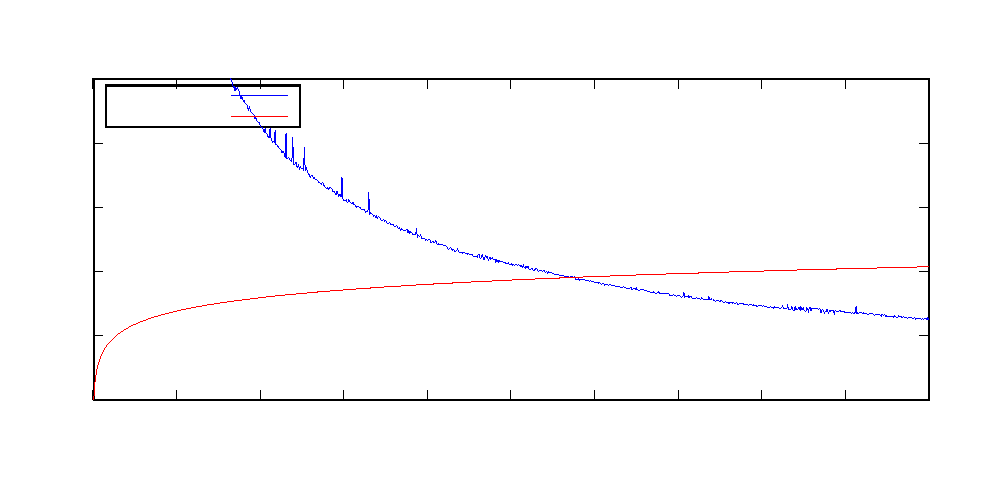
\includegraphics{problema1-instancias-aleatorias-logn}}%
    \gplfronttext
  \end{picture}%
\endgroup

  \caption{Instancias aleatorias ($log(n)$)}
\end{figure}

\begin{figure}[H]
  \centering
  % GNUPLOT: LaTeX picture with Postscript
\begingroup
  \makeatletter
  \providecommand\color[2][]{%
    \GenericError{(gnuplot) \space\space\space\@spaces}{%
      Package color not loaded in conjunction with
      terminal option `colourtext'%
    }{See the gnuplot documentation for explanation.%
    }{Either use 'blacktext' in gnuplot or load the package
      color.sty in LaTeX.}%
    \renewcommand\color[2][]{}%
  }%
  \providecommand\includegraphics[2][]{%
    \GenericError{(gnuplot) \space\space\space\@spaces}{%
      Package graphicx or graphics not loaded%
    }{See the gnuplot documentation for explanation.%
    }{The gnuplot epslatex terminal needs graphicx.sty or graphics.sty.}%
    \renewcommand\includegraphics[2][]{}%
  }%
  \providecommand\rotatebox[2]{#2}%
  \@ifundefined{ifGPcolor}{%
    \newif\ifGPcolor
    \GPcolorfalse
  }{}%
  \@ifundefined{ifGPblacktext}{%
    \newif\ifGPblacktext
    \GPblacktexttrue
  }{}%
  % define a \g@addto@macro without @ in the name:
  \let\gplgaddtomacro\g@addto@macro
  % define empty templates for all commands taking text:
  \gdef\gplbacktext{}%
  \gdef\gplfronttext{}%
  \makeatother
  \ifGPblacktext
    % no textcolor at all
    \def\colorrgb#1{}%
    \def\colorgray#1{}%
  \else
    % gray or color?
    \ifGPcolor
      \def\colorrgb#1{\color[rgb]{#1}}%
      \def\colorgray#1{\color[gray]{#1}}%
      \expandafter\def\csname LTw\endcsname{\color{white}}%
      \expandafter\def\csname LTb\endcsname{\color{black}}%
      \expandafter\def\csname LTa\endcsname{\color{black}}%
      \expandafter\def\csname LT0\endcsname{\color[rgb]{1,0,0}}%
      \expandafter\def\csname LT1\endcsname{\color[rgb]{0,1,0}}%
      \expandafter\def\csname LT2\endcsname{\color[rgb]{0,0,1}}%
      \expandafter\def\csname LT3\endcsname{\color[rgb]{1,0,1}}%
      \expandafter\def\csname LT4\endcsname{\color[rgb]{0,1,1}}%
      \expandafter\def\csname LT5\endcsname{\color[rgb]{1,1,0}}%
      \expandafter\def\csname LT6\endcsname{\color[rgb]{0,0,0}}%
      \expandafter\def\csname LT7\endcsname{\color[rgb]{1,0.3,0}}%
      \expandafter\def\csname LT8\endcsname{\color[rgb]{0.5,0.5,0.5}}%
    \else
      % gray
      \def\colorrgb#1{\color{black}}%
      \def\colorgray#1{\color[gray]{#1}}%
      \expandafter\def\csname LTw\endcsname{\color{white}}%
      \expandafter\def\csname LTb\endcsname{\color{black}}%
      \expandafter\def\csname LTa\endcsname{\color{black}}%
      \expandafter\def\csname LT0\endcsname{\color{black}}%
      \expandafter\def\csname LT1\endcsname{\color{black}}%
      \expandafter\def\csname LT2\endcsname{\color{black}}%
      \expandafter\def\csname LT3\endcsname{\color{black}}%
      \expandafter\def\csname LT4\endcsname{\color{black}}%
      \expandafter\def\csname LT5\endcsname{\color{black}}%
      \expandafter\def\csname LT6\endcsname{\color{black}}%
      \expandafter\def\csname LT7\endcsname{\color{black}}%
      \expandafter\def\csname LT8\endcsname{\color{black}}%
    \fi
  \fi
  \setlength{\unitlength}{0.0500bp}%
  \begin{picture}(7678.00,5280.00)%
    \gplgaddtomacro\gplbacktext{%
      \colorrgb{0.00,0.00,0.00}%
      \put(740,640){\makebox(0,0)[r]{\strut{}0}}%
      \colorrgb{0.00,0.00,0.00}%
      \put(740,1217){\makebox(0,0)[r]{\strut{}0.1}}%
      \colorrgb{0.00,0.00,0.00}%
      \put(740,1794){\makebox(0,0)[r]{\strut{}0.2}}%
      \colorrgb{0.00,0.00,0.00}%
      \put(740,2371){\makebox(0,0)[r]{\strut{}0.3}}%
      \colorrgb{0.00,0.00,0.00}%
      \put(740,2948){\makebox(0,0)[r]{\strut{}0.4}}%
      \colorrgb{0.00,0.00,0.00}%
      \put(740,3525){\makebox(0,0)[r]{\strut{}0.5}}%
      \colorrgb{0.00,0.00,0.00}%
      \put(740,4102){\makebox(0,0)[r]{\strut{}0.6}}%
      \colorrgb{0.00,0.00,0.00}%
      \put(740,4679){\makebox(0,0)[r]{\strut{}0.7}}%
      \colorrgb{0.00,0.00,0.00}%
      \put(860,440){\makebox(0,0){\strut{}100}}%
      \colorrgb{0.00,0.00,0.00}%
      \put(1666,440){\makebox(0,0){\strut{}200}}%
      \colorrgb{0.00,0.00,0.00}%
      \put(2472,440){\makebox(0,0){\strut{}300}}%
      \colorrgb{0.00,0.00,0.00}%
      \put(3278,440){\makebox(0,0){\strut{}400}}%
      \colorrgb{0.00,0.00,0.00}%
      \put(4084,440){\makebox(0,0){\strut{}500}}%
      \colorrgb{0.00,0.00,0.00}%
      \put(4891,440){\makebox(0,0){\strut{}600}}%
      \colorrgb{0.00,0.00,0.00}%
      \put(5697,440){\makebox(0,0){\strut{}700}}%
      \colorrgb{0.00,0.00,0.00}%
      \put(6503,440){\makebox(0,0){\strut{}800}}%
      \colorrgb{0.00,0.00,0.00}%
      \put(7309,440){\makebox(0,0){\strut{}900}}%
      \colorrgb{0.00,0.00,0.00}%
      \put(160,2659){\rotatebox{90}{\makebox(0,0){\strut{}Tiempo de ejecuci\'on [$mS$]}}}%
      \colorrgb{0.00,0.00,0.00}%
      \put(4088,140){\makebox(0,0){\strut{}$n$ (tama\~no del problema)}}%
      \csname LTb\endcsname%
      \put(4088,4979){\makebox(0,0){\strut{}Instancias aleatorias ($n$)}}%
    }%
    \gplgaddtomacro\gplfronttext{%
      \csname LTb\endcsname%
      \put(2300,4516){\makebox(0,0)[r]{\strut{}$t_n / log(n)$}}%
      \csname LTb\endcsname%
      \put(2300,4316){\makebox(0,0)[r]{\strut{}$n$}}%
    }%
    \gplbacktext
    \put(0,0){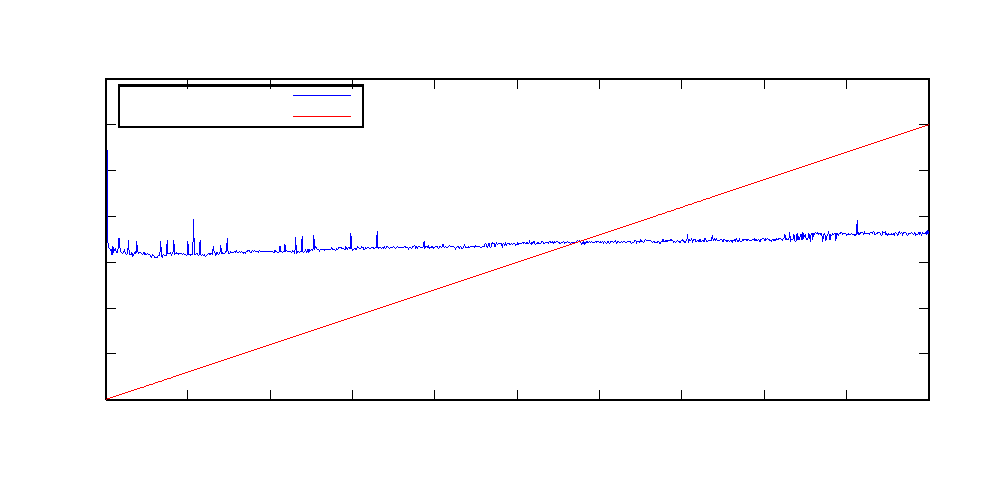
\includegraphics{problema1-instancias-aleatorias-n}}%
    \gplfronttext
  \end{picture}%
\endgroup

  \caption{Instancias aleatorias ($n$)}
\end{figure}


%%%%%%%%%%%%%%%%%%%%%%%%%%%%%%%%%%%%%%%%%%%%%%%%%%%%%%%%%%%%%%%%%%%%%%%%%%%%%%%
%% Problema 2: Profesores visitantes                                         %%
%%%%%%%%%%%%%%%%%%%%%%%%%%%%%%%%%%%%%%%%%%%%%%%%%%%%%%%%%%%%%%%%%%%%%%%%%%%%%%%


\newpage

\section{Problema 2: Profesores visitantes}

Dado un conjunto de $n$ cursos con una fecha de inicio y una fecha de finalización, se nos pide hallar el subconjunto con mayor cantidad de cursos tales que ningún curso se solapa con otro.

Se representa cada curso con una tupla $(i, f)$, donde $i$ y $f$ son las fechas de inicio y finalización del curso, respectivamente, tales que $i \leq f$.

Decimos que dos cursos $(i_1, f_1)$ y $(i_2, f_2)$ con $f_1 \leq f_2$ se solapan si y sólo si $f_1 \geq i_2$.

Formalmente, dado un conjunto de cursos $C = \{ (i_1, f_1), \ldots, (i_n, f_n) \}$, se nos pide hallar un subconjunto $S \subseteq C$ sin cursos solapados, tal que para cualquier otro $S' \subseteq C$ sin cursos solapados, vale que $|S| \geq |S'|$.

El problema debe ser resuelto con una cota de complejidad temporal \textbf{estrictamente mejor} que $O(n^2)$.

Algunas instancias del problema y sus soluciones:

\textbf{Entrada}: $\{(4, 4), (1, 3), (2, 5)\}$.\\
\textbf{Salida}: $\{(1, 3), (4, 4)\}$.

\textbf{Entrada}: $\{(4, 10), (5, 6), (2, 3), (7, 8), (3, 4), (1, 15)\}$.\\
\textbf{Salida}: $\{(2, 3), (5, 6), (7, 8)\}$ ó $\{(3, 4), (5, 6), (7, 8)\}$; cualquiera de las dos son correctas.

\textbf{Entrada}: $\{(1, 2)\}$.\\
\textbf{Salida}: $\{(1, 2)\}$.

\textbf{Entrada}: $\emptyset$.\\
\textbf{Salida}: $\emptyset$.


\subsection{Solución}

Sea $C = \{ (i_1, f_1), \ldots, (i_n, f_n) \}$ el conjunto con los $n$ cursos ordenados por fecha de finalización en forma creciente ($i < j \Rightarrow f_i \leq f_j$), y sea $S = \emptyset$ una solución del problema, inicialmente vacía.

Recorremos los cursos $c_j \in C$ (con $j = 1, \ldots, n$) en el orden anterior, realizando una de las siguientes acciones para cada $c_j$:

\begin{itemize}
    \item{
        Si $j = 1$, incluímos $c_1 = (i_1, f_1)$ en la solución: $S = \{ (i_1, f_1) \}$.
    }
    \item{
        Si $j > 1$ y $c_j = (i_j, f_j)$ \textbf{no se solapa} con el último curso agregado a la solución, lo incluímos en la misma: $S = S \cup \{ (i_j, f_j) \}$.
    }
    \item{
        En caso contrario, ignoramos $c_j$.
    }
\end{itemize}

Finalmente devolvemos la solución $S$ hallada.

En el pseudocódigo a continuación, $C$ denota el conjunto con la oferta de $n$ cursos $\{ (i_1, f_1), \ldots, (i_n, f_n) \}$.

\begin{pseudo}
    \Procedure{Profesores-visitantes}{$C$}
        \If{$|C| < 2$}
            \State{\Return{$C$}}                                \Ode{1}
        \Else
            \State{Ordenar $C$ por fecha de finalización
                   en forma creciente.}                         \Ode{n * log(n)}
            \State{$S = \{(i_1, j_1)\}$}                        \Ode{1}
            \State{$k = 1$}                                     \Ode{1}
            \For{$j = 2$ \To $|C|$}                             \Ode{n}
                \If{$i_j > f_k$}                                \Ode{1}
                    \State{$S = S \cup \{ (i_j, f_j) \}$}       \Ode{1}
                    \State{$k = j$}                             \Ode{1}
                \EndIf
            \EndFor
            \State{\Return{$S$}}
        \EndIf
    \EndProcedure 
\end{pseudo}


\subsection{Complejidad}

El algoritmo corre en tiempo $O(n*log(n))$, donde $n$ es la cantidad de cursos.

Demostración: para el caso no trivial ($n > 1$) se ordenan los cursos en $O(n * log(n))$, luego se recorre cada curso y se decide si se lo incluye en la solución o no, con costo $n * O(1)$. La complejidad total resulta $O(n * log(n)) + n * O(1) = O(n * log(n) + n) = O(n * log(n))$. Para el caso trivial, se devuelve el conjunto de cursos intacto en tiempo constante.


\subsection{Correctitud}

El algoritmo incluye en la solución el curso que termina primero, descarta los cursos que se solapan con este y repite lo anterior con los cursos restantes hasta que no queden más cursos.

Para que el procedimiento anterior arroje una solución válida, tiene que cumplirse que para cualquier instancia del problema, el curso con fecha de finalización más temprana siempre sea parte de alguna solución. Si esto se cumple, podemos incluir dicho curso en nuestra solución, descartar todos los cursos que se solapan con este, resolver el subproblema resultante aplicando el mismo razonamiento e incluir la solución del subproblema en la solución al problema original.

El teorema a continuación muestra que la suposición anterior es de hecho cierta.

\newtheorem*{teorema-ej2}{Teorema}

\begin{teorema-ej2}
    Sea $C = \{ (i_1, f_1), \ldots, (i_n, f_n) \}$ la oferta de $n$ cursos ordenados por fecha de finalización de forma creciente. Entonces el curso $(i_1, f_1)$ está incluido en algún subconjunto de $C$ tal que sus cursos no se solapan entre sí y su cardinalidad es máxima.
\end{teorema-ej2}

\begin{proof}
    Sea $S$ algún subconjunto $\subseteq C$ tal que sus cursos no se solapan entre sí y su cardinalidad es máxima, y sea $(i_j, f_j)$ el curso $\in S$ con fecha de finalización más temprana.

    Si $(i_j, f_j) = (i_1, f_1)$ terminamos la demostración, pues hemos mostrado que $(i_1, f_1)$ está incluido en algún subconjunto de $C$ tal que sus cursos no se solapan entre sí y su cardinalidad es máxima.

    Si $(i_j, f_j) \neq (i_1, f_1)$, entonces sea $S' = S - \{ (i_j, f_j) \} \cup \{ (i_1, f_1) \}$ el conjunto $S$ al que le reemplazamos $(i_j, f_j)$ por $(i_1, f_1)$. Los cursos en $S'$ no se solapan entre sí pues:

    \begin{itemize}[nolistsep]
        \item{los cursos en $S$ no se solapan entre sí,}
        \item{$(i_j, f_j)$ es la actividad en $S$ que termina primero, y}
        \item{$f_1 \leq f_j$.}
    \end{itemize}

    Como $|S'| = |S|$, concluímos que $S'$ es un subconjunto de $C$ tal que sus cursos no se solapan entre sí y su cardinalidad es máxima, y $(i_1, f_1)$ está incluido en $S'$, como queríamos ver.
\end{proof}


\subsubsection{Peor caso}

\begin{figure}[H]
  \centering
  % GNUPLOT: LaTeX picture with Postscript
\begingroup
  \makeatletter
  \providecommand\color[2][]{%
    \GenericError{(gnuplot) \space\space\space\@spaces}{%
      Package color not loaded in conjunction with
      terminal option `colourtext'%
    }{See the gnuplot documentation for explanation.%
    }{Either use 'blacktext' in gnuplot or load the package
      color.sty in LaTeX.}%
    \renewcommand\color[2][]{}%
  }%
  \providecommand\includegraphics[2][]{%
    \GenericError{(gnuplot) \space\space\space\@spaces}{%
      Package graphicx or graphics not loaded%
    }{See the gnuplot documentation for explanation.%
    }{The gnuplot epslatex terminal needs graphicx.sty or graphics.sty.}%
    \renewcommand\includegraphics[2][]{}%
  }%
  \providecommand\rotatebox[2]{#2}%
  \@ifundefined{ifGPcolor}{%
    \newif\ifGPcolor
    \GPcolorfalse
  }{}%
  \@ifundefined{ifGPblacktext}{%
    \newif\ifGPblacktext
    \GPblacktexttrue
  }{}%
  % define a \g@addto@macro without @ in the name:
  \let\gplgaddtomacro\g@addto@macro
  % define empty templates for all commands taking text:
  \gdef\gplbacktext{}%
  \gdef\gplfronttext{}%
  \makeatother
  \ifGPblacktext
    % no textcolor at all
    \def\colorrgb#1{}%
    \def\colorgray#1{}%
  \else
    % gray or color?
    \ifGPcolor
      \def\colorrgb#1{\color[rgb]{#1}}%
      \def\colorgray#1{\color[gray]{#1}}%
      \expandafter\def\csname LTw\endcsname{\color{white}}%
      \expandafter\def\csname LTb\endcsname{\color{black}}%
      \expandafter\def\csname LTa\endcsname{\color{black}}%
      \expandafter\def\csname LT0\endcsname{\color[rgb]{1,0,0}}%
      \expandafter\def\csname LT1\endcsname{\color[rgb]{0,1,0}}%
      \expandafter\def\csname LT2\endcsname{\color[rgb]{0,0,1}}%
      \expandafter\def\csname LT3\endcsname{\color[rgb]{1,0,1}}%
      \expandafter\def\csname LT4\endcsname{\color[rgb]{0,1,1}}%
      \expandafter\def\csname LT5\endcsname{\color[rgb]{1,1,0}}%
      \expandafter\def\csname LT6\endcsname{\color[rgb]{0,0,0}}%
      \expandafter\def\csname LT7\endcsname{\color[rgb]{1,0.3,0}}%
      \expandafter\def\csname LT8\endcsname{\color[rgb]{0.5,0.5,0.5}}%
    \else
      % gray
      \def\colorrgb#1{\color{black}}%
      \def\colorgray#1{\color[gray]{#1}}%
      \expandafter\def\csname LTw\endcsname{\color{white}}%
      \expandafter\def\csname LTb\endcsname{\color{black}}%
      \expandafter\def\csname LTa\endcsname{\color{black}}%
      \expandafter\def\csname LT0\endcsname{\color{black}}%
      \expandafter\def\csname LT1\endcsname{\color{black}}%
      \expandafter\def\csname LT2\endcsname{\color{black}}%
      \expandafter\def\csname LT3\endcsname{\color{black}}%
      \expandafter\def\csname LT4\endcsname{\color{black}}%
      \expandafter\def\csname LT5\endcsname{\color{black}}%
      \expandafter\def\csname LT6\endcsname{\color{black}}%
      \expandafter\def\csname LT7\endcsname{\color{black}}%
      \expandafter\def\csname LT8\endcsname{\color{black}}%
    \fi
  \fi
  \setlength{\unitlength}{0.0500bp}%
  \begin{picture}(7678.00,5280.00)%
    \gplgaddtomacro\gplbacktext{%
      \colorrgb{0.00,0.00,0.00}%
      \put(740,640){\makebox(0,0)[r]{\strut{}0}}%
      \colorrgb{0.00,0.00,0.00}%
      \put(740,1313){\makebox(0,0)[r]{\strut{}0.5}}%
      \colorrgb{0.00,0.00,0.00}%
      \put(740,1986){\makebox(0,0)[r]{\strut{}1}}%
      \colorrgb{0.00,0.00,0.00}%
      \put(740,2660){\makebox(0,0)[r]{\strut{}1.5}}%
      \colorrgb{0.00,0.00,0.00}%
      \put(740,3333){\makebox(0,0)[r]{\strut{}2}}%
      \colorrgb{0.00,0.00,0.00}%
      \put(740,4006){\makebox(0,0)[r]{\strut{}2.5}}%
      \colorrgb{0.00,0.00,0.00}%
      \put(740,4679){\makebox(0,0)[r]{\strut{}3}}%
      \colorrgb{0.00,0.00,0.00}%
      \put(854,440){\makebox(0,0){\strut{}0}}%
      \colorrgb{0.00,0.00,0.00}%
      \put(1500,440){\makebox(0,0){\strut{}100}}%
      \colorrgb{0.00,0.00,0.00}%
      \put(2146,440){\makebox(0,0){\strut{}200}}%
      \colorrgb{0.00,0.00,0.00}%
      \put(2793,440){\makebox(0,0){\strut{}300}}%
      \colorrgb{0.00,0.00,0.00}%
      \put(3439,440){\makebox(0,0){\strut{}400}}%
      \colorrgb{0.00,0.00,0.00}%
      \put(4085,440){\makebox(0,0){\strut{}500}}%
      \colorrgb{0.00,0.00,0.00}%
      \put(4732,440){\makebox(0,0){\strut{}600}}%
      \colorrgb{0.00,0.00,0.00}%
      \put(5378,440){\makebox(0,0){\strut{}700}}%
      \colorrgb{0.00,0.00,0.00}%
      \put(6024,440){\makebox(0,0){\strut{}800}}%
      \colorrgb{0.00,0.00,0.00}%
      \put(6671,440){\makebox(0,0){\strut{}900}}%
      \colorrgb{0.00,0.00,0.00}%
      \put(7317,440){\makebox(0,0){\strut{}1000}}%
      \colorrgb{0.00,0.00,0.00}%
      \put(160,2659){\rotatebox{90}{\makebox(0,0){\strut{}Tiempo de ejecuci\'on [$mS$]}}}%
      \colorrgb{0.00,0.00,0.00}%
      \put(4088,140){\makebox(0,0){\strut{}$n$ (tama\~no del problema)}}%
      \csname LTb\endcsname%
      \put(4088,4979){\makebox(0,0){\strut{}Peor caso}}%
    }%
    \gplgaddtomacro\gplfronttext{%
      \csname LTb\endcsname%
      \put(2180,4516){\makebox(0,0)[r]{\strut{}$t_n$}}%
      \csname LTb\endcsname%
      \put(2180,4316){\makebox(0,0)[r]{\strut{}$n * log(n)$}}%
    }%
    \gplbacktext
    \put(0,0){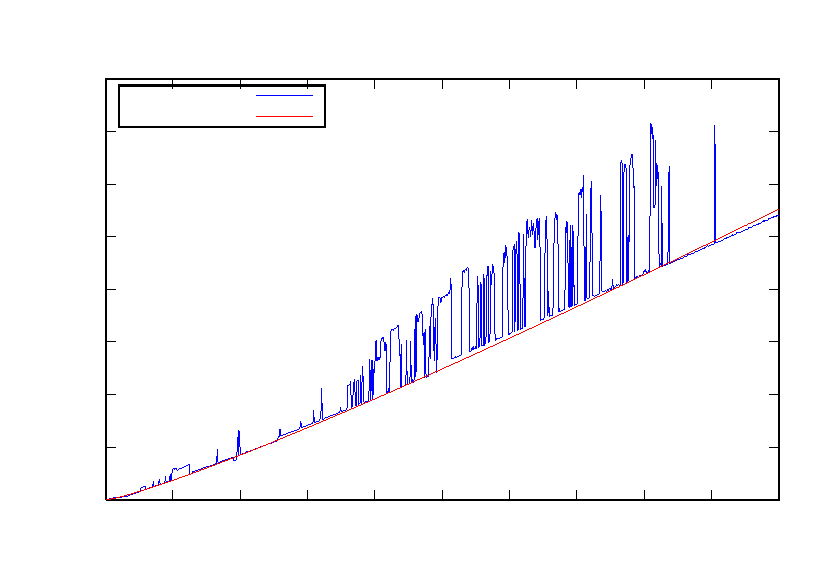
\includegraphics{problema2-peor-caso}}%
    \gplfronttext
  \end{picture}%
\endgroup

  \caption{Peor caso}
\end{figure}

\begin{figure}[H]
  \centering
  % GNUPLOT: LaTeX picture with Postscript
\begingroup
  \makeatletter
  \providecommand\color[2][]{%
    \GenericError{(gnuplot) \space\space\space\@spaces}{%
      Package color not loaded in conjunction with
      terminal option `colourtext'%
    }{See the gnuplot documentation for explanation.%
    }{Either use 'blacktext' in gnuplot or load the package
      color.sty in LaTeX.}%
    \renewcommand\color[2][]{}%
  }%
  \providecommand\includegraphics[2][]{%
    \GenericError{(gnuplot) \space\space\space\@spaces}{%
      Package graphicx or graphics not loaded%
    }{See the gnuplot documentation for explanation.%
    }{The gnuplot epslatex terminal needs graphicx.sty or graphics.sty.}%
    \renewcommand\includegraphics[2][]{}%
  }%
  \providecommand\rotatebox[2]{#2}%
  \@ifundefined{ifGPcolor}{%
    \newif\ifGPcolor
    \GPcolorfalse
  }{}%
  \@ifundefined{ifGPblacktext}{%
    \newif\ifGPblacktext
    \GPblacktexttrue
  }{}%
  % define a \g@addto@macro without @ in the name:
  \let\gplgaddtomacro\g@addto@macro
  % define empty templates for all commands taking text:
  \gdef\gplbacktext{}%
  \gdef\gplfronttext{}%
  \makeatother
  \ifGPblacktext
    % no textcolor at all
    \def\colorrgb#1{}%
    \def\colorgray#1{}%
  \else
    % gray or color?
    \ifGPcolor
      \def\colorrgb#1{\color[rgb]{#1}}%
      \def\colorgray#1{\color[gray]{#1}}%
      \expandafter\def\csname LTw\endcsname{\color{white}}%
      \expandafter\def\csname LTb\endcsname{\color{black}}%
      \expandafter\def\csname LTa\endcsname{\color{black}}%
      \expandafter\def\csname LT0\endcsname{\color[rgb]{1,0,0}}%
      \expandafter\def\csname LT1\endcsname{\color[rgb]{0,1,0}}%
      \expandafter\def\csname LT2\endcsname{\color[rgb]{0,0,1}}%
      \expandafter\def\csname LT3\endcsname{\color[rgb]{1,0,1}}%
      \expandafter\def\csname LT4\endcsname{\color[rgb]{0,1,1}}%
      \expandafter\def\csname LT5\endcsname{\color[rgb]{1,1,0}}%
      \expandafter\def\csname LT6\endcsname{\color[rgb]{0,0,0}}%
      \expandafter\def\csname LT7\endcsname{\color[rgb]{1,0.3,0}}%
      \expandafter\def\csname LT8\endcsname{\color[rgb]{0.5,0.5,0.5}}%
    \else
      % gray
      \def\colorrgb#1{\color{black}}%
      \def\colorgray#1{\color[gray]{#1}}%
      \expandafter\def\csname LTw\endcsname{\color{white}}%
      \expandafter\def\csname LTb\endcsname{\color{black}}%
      \expandafter\def\csname LTa\endcsname{\color{black}}%
      \expandafter\def\csname LT0\endcsname{\color{black}}%
      \expandafter\def\csname LT1\endcsname{\color{black}}%
      \expandafter\def\csname LT2\endcsname{\color{black}}%
      \expandafter\def\csname LT3\endcsname{\color{black}}%
      \expandafter\def\csname LT4\endcsname{\color{black}}%
      \expandafter\def\csname LT5\endcsname{\color{black}}%
      \expandafter\def\csname LT6\endcsname{\color{black}}%
      \expandafter\def\csname LT7\endcsname{\color{black}}%
      \expandafter\def\csname LT8\endcsname{\color{black}}%
    \fi
  \fi
  \setlength{\unitlength}{0.0500bp}%
  \begin{picture}(9118.00,4320.00)%
    \gplgaddtomacro\gplbacktext{%
      \colorrgb{0.00,0.00,0.00}%
      \put(740,640){\makebox(0,0)[r]{\strut{}0}}%
      \colorrgb{0.00,0.00,0.00}%
      \put(740,1153){\makebox(0,0)[r]{\strut{}0.5}}%
      \colorrgb{0.00,0.00,0.00}%
      \put(740,1666){\makebox(0,0)[r]{\strut{}1}}%
      \colorrgb{0.00,0.00,0.00}%
      \put(740,2180){\makebox(0,0)[r]{\strut{}1.5}}%
      \colorrgb{0.00,0.00,0.00}%
      \put(740,2693){\makebox(0,0)[r]{\strut{}2}}%
      \colorrgb{0.00,0.00,0.00}%
      \put(740,3206){\makebox(0,0)[r]{\strut{}2.5}}%
      \colorrgb{0.00,0.00,0.00}%
      \put(740,3719){\makebox(0,0)[r]{\strut{}3}}%
      \colorrgb{0.00,0.00,0.00}%
      \put(852,440){\makebox(0,0){\strut{}0}}%
      \colorrgb{0.00,0.00,0.00}%
      \put(1643,440){\makebox(0,0){\strut{}100}}%
      \colorrgb{0.00,0.00,0.00}%
      \put(2433,440){\makebox(0,0){\strut{}200}}%
      \colorrgb{0.00,0.00,0.00}%
      \put(3224,440){\makebox(0,0){\strut{}300}}%
      \colorrgb{0.00,0.00,0.00}%
      \put(4014,440){\makebox(0,0){\strut{}400}}%
      \colorrgb{0.00,0.00,0.00}%
      \put(4805,440){\makebox(0,0){\strut{}500}}%
      \colorrgb{0.00,0.00,0.00}%
      \put(5595,440){\makebox(0,0){\strut{}600}}%
      \colorrgb{0.00,0.00,0.00}%
      \put(6386,440){\makebox(0,0){\strut{}700}}%
      \colorrgb{0.00,0.00,0.00}%
      \put(7176,440){\makebox(0,0){\strut{}800}}%
      \colorrgb{0.00,0.00,0.00}%
      \put(7967,440){\makebox(0,0){\strut{}900}}%
      \colorrgb{0.00,0.00,0.00}%
      \put(8757,440){\makebox(0,0){\strut{}1000}}%
      \colorrgb{0.00,0.00,0.00}%
      \put(160,2179){\rotatebox{90}{\makebox(0,0){\strut{}Tiempo [$\mu S$]}}}%
      \colorrgb{0.00,0.00,0.00}%
      \put(4808,140){\makebox(0,0){\strut{}$n$ (tama\~no del problema)}}%
      \csname LTb\endcsname%
      \put(4808,4019){\makebox(0,0){\strut{}Tiempo de ejecuci\'on dividido por $n$}}%
    }%
    \gplgaddtomacro\gplfronttext{%
      \csname LTb\endcsname%
      \put(2060,3556){\makebox(0,0)[r]{\strut{}$T(n) / n$}}%
      \csname LTb\endcsname%
      \put(2060,3356){\makebox(0,0)[r]{\strut{}$O(log(n))$}}%
    }%
    \gplbacktext
    \put(0,0){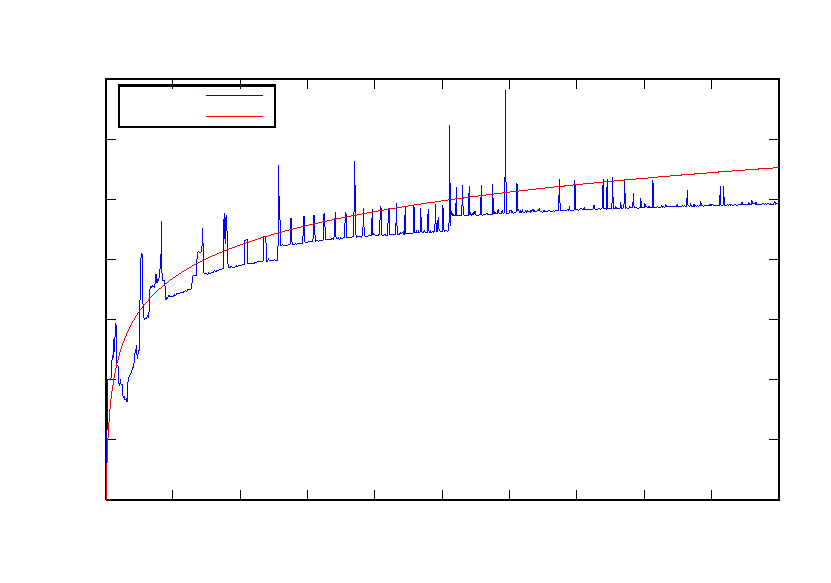
\includegraphics{problema2-peor-caso-logn}}%
    \gplfronttext
  \end{picture}%
\endgroup

  \caption{Peor caso ($log(n)$)}
\end{figure}

\begin{figure}[H]
  \centering
  % GNUPLOT: LaTeX picture with Postscript
\begingroup
  \makeatletter
  \providecommand\color[2][]{%
    \GenericError{(gnuplot) \space\space\space\@spaces}{%
      Package color not loaded in conjunction with
      terminal option `colourtext'%
    }{See the gnuplot documentation for explanation.%
    }{Either use 'blacktext' in gnuplot or load the package
      color.sty in LaTeX.}%
    \renewcommand\color[2][]{}%
  }%
  \providecommand\includegraphics[2][]{%
    \GenericError{(gnuplot) \space\space\space\@spaces}{%
      Package graphicx or graphics not loaded%
    }{See the gnuplot documentation for explanation.%
    }{The gnuplot epslatex terminal needs graphicx.sty or graphics.sty.}%
    \renewcommand\includegraphics[2][]{}%
  }%
  \providecommand\rotatebox[2]{#2}%
  \@ifundefined{ifGPcolor}{%
    \newif\ifGPcolor
    \GPcolorfalse
  }{}%
  \@ifundefined{ifGPblacktext}{%
    \newif\ifGPblacktext
    \GPblacktexttrue
  }{}%
  % define a \g@addto@macro without @ in the name:
  \let\gplgaddtomacro\g@addto@macro
  % define empty templates for all commands taking text:
  \gdef\gplbacktext{}%
  \gdef\gplfronttext{}%
  \makeatother
  \ifGPblacktext
    % no textcolor at all
    \def\colorrgb#1{}%
    \def\colorgray#1{}%
  \else
    % gray or color?
    \ifGPcolor
      \def\colorrgb#1{\color[rgb]{#1}}%
      \def\colorgray#1{\color[gray]{#1}}%
      \expandafter\def\csname LTw\endcsname{\color{white}}%
      \expandafter\def\csname LTb\endcsname{\color{black}}%
      \expandafter\def\csname LTa\endcsname{\color{black}}%
      \expandafter\def\csname LT0\endcsname{\color[rgb]{1,0,0}}%
      \expandafter\def\csname LT1\endcsname{\color[rgb]{0,1,0}}%
      \expandafter\def\csname LT2\endcsname{\color[rgb]{0,0,1}}%
      \expandafter\def\csname LT3\endcsname{\color[rgb]{1,0,1}}%
      \expandafter\def\csname LT4\endcsname{\color[rgb]{0,1,1}}%
      \expandafter\def\csname LT5\endcsname{\color[rgb]{1,1,0}}%
      \expandafter\def\csname LT6\endcsname{\color[rgb]{0,0,0}}%
      \expandafter\def\csname LT7\endcsname{\color[rgb]{1,0.3,0}}%
      \expandafter\def\csname LT8\endcsname{\color[rgb]{0.5,0.5,0.5}}%
    \else
      % gray
      \def\colorrgb#1{\color{black}}%
      \def\colorgray#1{\color[gray]{#1}}%
      \expandafter\def\csname LTw\endcsname{\color{white}}%
      \expandafter\def\csname LTb\endcsname{\color{black}}%
      \expandafter\def\csname LTa\endcsname{\color{black}}%
      \expandafter\def\csname LT0\endcsname{\color{black}}%
      \expandafter\def\csname LT1\endcsname{\color{black}}%
      \expandafter\def\csname LT2\endcsname{\color{black}}%
      \expandafter\def\csname LT3\endcsname{\color{black}}%
      \expandafter\def\csname LT4\endcsname{\color{black}}%
      \expandafter\def\csname LT5\endcsname{\color{black}}%
      \expandafter\def\csname LT6\endcsname{\color{black}}%
      \expandafter\def\csname LT7\endcsname{\color{black}}%
      \expandafter\def\csname LT8\endcsname{\color{black}}%
    \fi
  \fi
  \setlength{\unitlength}{0.0500bp}%
  \begin{picture}(9118.00,4320.00)%
    \gplgaddtomacro\gplbacktext{%
      \colorrgb{0.00,0.00,0.00}%
      \put(860,640){\makebox(0,0)[r]{\strut{}0}}%
      \colorrgb{0.00,0.00,0.00}%
      \put(860,1025){\makebox(0,0)[r]{\strut{}0.05}}%
      \colorrgb{0.00,0.00,0.00}%
      \put(860,1410){\makebox(0,0)[r]{\strut{}0.1}}%
      \colorrgb{0.00,0.00,0.00}%
      \put(860,1795){\makebox(0,0)[r]{\strut{}0.15}}%
      \colorrgb{0.00,0.00,0.00}%
      \put(860,2180){\makebox(0,0)[r]{\strut{}0.2}}%
      \colorrgb{0.00,0.00,0.00}%
      \put(860,2564){\makebox(0,0)[r]{\strut{}0.25}}%
      \colorrgb{0.00,0.00,0.00}%
      \put(860,2949){\makebox(0,0)[r]{\strut{}0.3}}%
      \colorrgb{0.00,0.00,0.00}%
      \put(860,3334){\makebox(0,0)[r]{\strut{}0.35}}%
      \colorrgb{0.00,0.00,0.00}%
      \put(860,3719){\makebox(0,0)[r]{\strut{}0.4}}%
      \colorrgb{0.00,0.00,0.00}%
      \put(972,440){\makebox(0,0){\strut{}0}}%
      \colorrgb{0.00,0.00,0.00}%
      \put(1751,440){\makebox(0,0){\strut{}100}}%
      \colorrgb{0.00,0.00,0.00}%
      \put(2529,440){\makebox(0,0){\strut{}200}}%
      \colorrgb{0.00,0.00,0.00}%
      \put(3308,440){\makebox(0,0){\strut{}300}}%
      \colorrgb{0.00,0.00,0.00}%
      \put(4086,440){\makebox(0,0){\strut{}400}}%
      \colorrgb{0.00,0.00,0.00}%
      \put(4865,440){\makebox(0,0){\strut{}500}}%
      \colorrgb{0.00,0.00,0.00}%
      \put(5643,440){\makebox(0,0){\strut{}600}}%
      \colorrgb{0.00,0.00,0.00}%
      \put(6422,440){\makebox(0,0){\strut{}700}}%
      \colorrgb{0.00,0.00,0.00}%
      \put(7200,440){\makebox(0,0){\strut{}800}}%
      \colorrgb{0.00,0.00,0.00}%
      \put(7979,440){\makebox(0,0){\strut{}900}}%
      \colorrgb{0.00,0.00,0.00}%
      \put(8757,440){\makebox(0,0){\strut{}1000}}%
      \colorrgb{0.00,0.00,0.00}%
      \put(160,2179){\rotatebox{90}{\makebox(0,0){\strut{}Tiempo [$mS$]}}}%
      \colorrgb{0.00,0.00,0.00}%
      \put(4868,140){\makebox(0,0){\strut{}$n$ (tama\~no del problema)}}%
      \csname LTb\endcsname%
      \put(4868,4019){\makebox(0,0){\strut{}Tiempo de ejecuci\'on dividido por $log(n)$}}%
    }%
    \gplgaddtomacro\gplfronttext{%
      \csname LTb\endcsname%
      \put(2420,3556){\makebox(0,0)[r]{\strut{}$t_n / log(n)$}}%
      \csname LTb\endcsname%
      \put(2420,3356){\makebox(0,0)[r]{\strut{}$n$}}%
    }%
    \gplbacktext
    \put(0,0){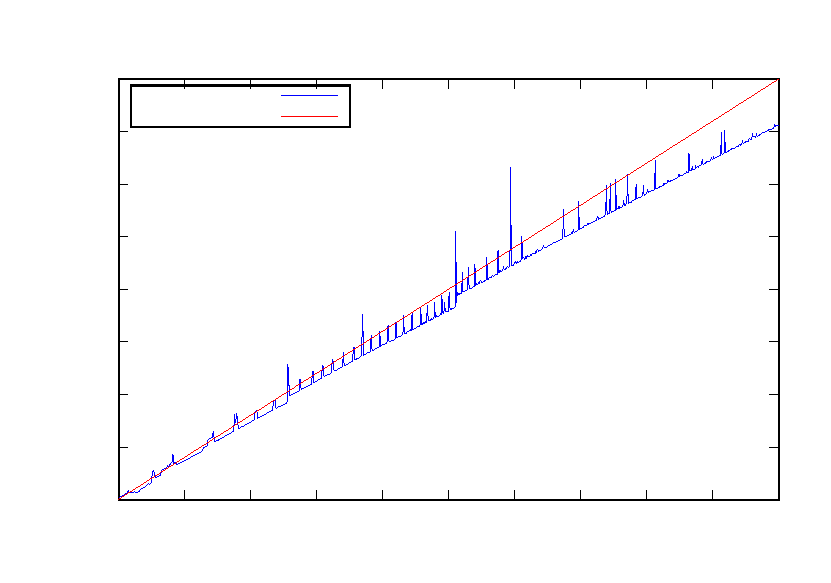
\includegraphics{problema2-peor-caso-n}}%
    \gplfronttext
  \end{picture}%
\endgroup

  \caption{Peor caso ($n$)}
\end{figure}


\subsubsection{Mejor caso}

\begin{figure}[H]
  \centering
  % GNUPLOT: LaTeX picture with Postscript
\begingroup
  \makeatletter
  \providecommand\color[2][]{%
    \GenericError{(gnuplot) \space\space\space\@spaces}{%
      Package color not loaded in conjunction with
      terminal option `colourtext'%
    }{See the gnuplot documentation for explanation.%
    }{Either use 'blacktext' in gnuplot or load the package
      color.sty in LaTeX.}%
    \renewcommand\color[2][]{}%
  }%
  \providecommand\includegraphics[2][]{%
    \GenericError{(gnuplot) \space\space\space\@spaces}{%
      Package graphicx or graphics not loaded%
    }{See the gnuplot documentation for explanation.%
    }{The gnuplot epslatex terminal needs graphicx.sty or graphics.sty.}%
    \renewcommand\includegraphics[2][]{}%
  }%
  \providecommand\rotatebox[2]{#2}%
  \@ifundefined{ifGPcolor}{%
    \newif\ifGPcolor
    \GPcolorfalse
  }{}%
  \@ifundefined{ifGPblacktext}{%
    \newif\ifGPblacktext
    \GPblacktexttrue
  }{}%
  % define a \g@addto@macro without @ in the name:
  \let\gplgaddtomacro\g@addto@macro
  % define empty templates for all commands taking text:
  \gdef\gplbacktext{}%
  \gdef\gplfronttext{}%
  \makeatother
  \ifGPblacktext
    % no textcolor at all
    \def\colorrgb#1{}%
    \def\colorgray#1{}%
  \else
    % gray or color?
    \ifGPcolor
      \def\colorrgb#1{\color[rgb]{#1}}%
      \def\colorgray#1{\color[gray]{#1}}%
      \expandafter\def\csname LTw\endcsname{\color{white}}%
      \expandafter\def\csname LTb\endcsname{\color{black}}%
      \expandafter\def\csname LTa\endcsname{\color{black}}%
      \expandafter\def\csname LT0\endcsname{\color[rgb]{1,0,0}}%
      \expandafter\def\csname LT1\endcsname{\color[rgb]{0,1,0}}%
      \expandafter\def\csname LT2\endcsname{\color[rgb]{0,0,1}}%
      \expandafter\def\csname LT3\endcsname{\color[rgb]{1,0,1}}%
      \expandafter\def\csname LT4\endcsname{\color[rgb]{0,1,1}}%
      \expandafter\def\csname LT5\endcsname{\color[rgb]{1,1,0}}%
      \expandafter\def\csname LT6\endcsname{\color[rgb]{0,0,0}}%
      \expandafter\def\csname LT7\endcsname{\color[rgb]{1,0.3,0}}%
      \expandafter\def\csname LT8\endcsname{\color[rgb]{0.5,0.5,0.5}}%
    \else
      % gray
      \def\colorrgb#1{\color{black}}%
      \def\colorgray#1{\color[gray]{#1}}%
      \expandafter\def\csname LTw\endcsname{\color{white}}%
      \expandafter\def\csname LTb\endcsname{\color{black}}%
      \expandafter\def\csname LTa\endcsname{\color{black}}%
      \expandafter\def\csname LT0\endcsname{\color{black}}%
      \expandafter\def\csname LT1\endcsname{\color{black}}%
      \expandafter\def\csname LT2\endcsname{\color{black}}%
      \expandafter\def\csname LT3\endcsname{\color{black}}%
      \expandafter\def\csname LT4\endcsname{\color{black}}%
      \expandafter\def\csname LT5\endcsname{\color{black}}%
      \expandafter\def\csname LT6\endcsname{\color{black}}%
      \expandafter\def\csname LT7\endcsname{\color{black}}%
      \expandafter\def\csname LT8\endcsname{\color{black}}%
    \fi
  \fi
  \setlength{\unitlength}{0.0500bp}%
  \begin{picture}(9118.00,4320.00)%
    \gplgaddtomacro\gplbacktext{%
      \colorrgb{0.00,0.00,0.00}%
      \put(740,640){\makebox(0,0)[r]{\strut{}0}}%
      \colorrgb{0.00,0.00,0.00}%
      \put(740,1256){\makebox(0,0)[r]{\strut{}0.2}}%
      \colorrgb{0.00,0.00,0.00}%
      \put(740,1872){\makebox(0,0)[r]{\strut{}0.4}}%
      \colorrgb{0.00,0.00,0.00}%
      \put(740,2487){\makebox(0,0)[r]{\strut{}0.6}}%
      \colorrgb{0.00,0.00,0.00}%
      \put(740,3103){\makebox(0,0)[r]{\strut{}0.8}}%
      \colorrgb{0.00,0.00,0.00}%
      \put(740,3719){\makebox(0,0)[r]{\strut{}1}}%
      \colorrgb{0.00,0.00,0.00}%
      \put(852,440){\makebox(0,0){\strut{}0}}%
      \colorrgb{0.00,0.00,0.00}%
      \put(1643,440){\makebox(0,0){\strut{}100}}%
      \colorrgb{0.00,0.00,0.00}%
      \put(2433,440){\makebox(0,0){\strut{}200}}%
      \colorrgb{0.00,0.00,0.00}%
      \put(3224,440){\makebox(0,0){\strut{}300}}%
      \colorrgb{0.00,0.00,0.00}%
      \put(4014,440){\makebox(0,0){\strut{}400}}%
      \colorrgb{0.00,0.00,0.00}%
      \put(4805,440){\makebox(0,0){\strut{}500}}%
      \colorrgb{0.00,0.00,0.00}%
      \put(5595,440){\makebox(0,0){\strut{}600}}%
      \colorrgb{0.00,0.00,0.00}%
      \put(6386,440){\makebox(0,0){\strut{}700}}%
      \colorrgb{0.00,0.00,0.00}%
      \put(7176,440){\makebox(0,0){\strut{}800}}%
      \colorrgb{0.00,0.00,0.00}%
      \put(7967,440){\makebox(0,0){\strut{}900}}%
      \colorrgb{0.00,0.00,0.00}%
      \put(8757,440){\makebox(0,0){\strut{}1000}}%
      \colorrgb{0.00,0.00,0.00}%
      \put(160,2179){\rotatebox{90}{\makebox(0,0){\strut{}Tiempo [$mS$]}}}%
      \colorrgb{0.00,0.00,0.00}%
      \put(4808,140){\makebox(0,0){\strut{}$n$ (tama\~no del problema)}}%
      \csname LTb\endcsname%
      \put(4808,4019){\makebox(0,0){\strut{}Tiempo de ejecuci\'on}}%
    }%
    \gplgaddtomacro\gplfronttext{%
      \csname LTb\endcsname%
      \put(2540,3556){\makebox(0,0)[r]{\strut{}$T(n)$}}%
      \csname LTb\endcsname%
      \put(2540,3356){\makebox(0,0)[r]{\strut{}$O(n * log(n))$}}%
    }%
    \gplbacktext
    \put(0,0){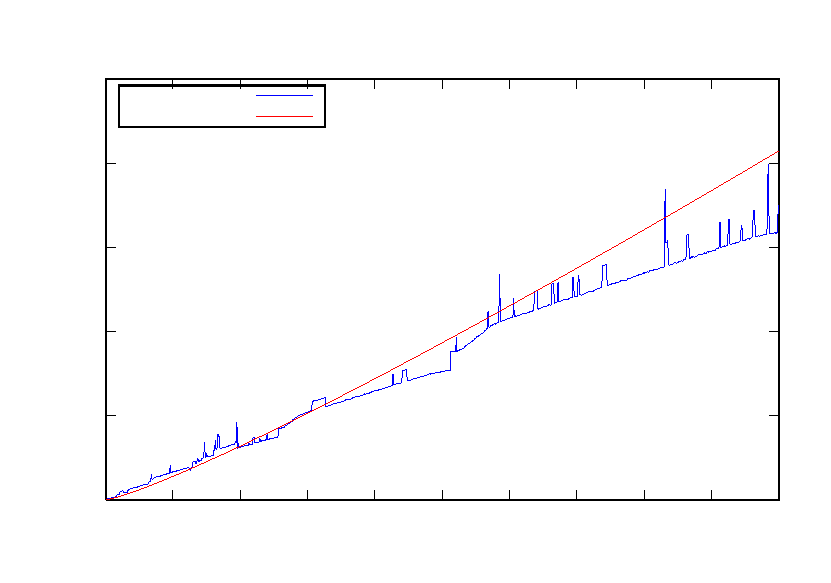
\includegraphics{problema2-mejor-caso}}%
    \gplfronttext
  \end{picture}%
\endgroup

  \caption{Mejor caso}
\end{figure}

\begin{figure}[H]
  \centering
  % GNUPLOT: LaTeX picture with Postscript
\begingroup
  \makeatletter
  \providecommand\color[2][]{%
    \GenericError{(gnuplot) \space\space\space\@spaces}{%
      Package color not loaded in conjunction with
      terminal option `colourtext'%
    }{See the gnuplot documentation for explanation.%
    }{Either use 'blacktext' in gnuplot or load the package
      color.sty in LaTeX.}%
    \renewcommand\color[2][]{}%
  }%
  \providecommand\includegraphics[2][]{%
    \GenericError{(gnuplot) \space\space\space\@spaces}{%
      Package graphicx or graphics not loaded%
    }{See the gnuplot documentation for explanation.%
    }{The gnuplot epslatex terminal needs graphicx.sty or graphics.sty.}%
    \renewcommand\includegraphics[2][]{}%
  }%
  \providecommand\rotatebox[2]{#2}%
  \@ifundefined{ifGPcolor}{%
    \newif\ifGPcolor
    \GPcolorfalse
  }{}%
  \@ifundefined{ifGPblacktext}{%
    \newif\ifGPblacktext
    \GPblacktexttrue
  }{}%
  % define a \g@addto@macro without @ in the name:
  \let\gplgaddtomacro\g@addto@macro
  % define empty templates for all commands taking text:
  \gdef\gplbacktext{}%
  \gdef\gplfronttext{}%
  \makeatother
  \ifGPblacktext
    % no textcolor at all
    \def\colorrgb#1{}%
    \def\colorgray#1{}%
  \else
    % gray or color?
    \ifGPcolor
      \def\colorrgb#1{\color[rgb]{#1}}%
      \def\colorgray#1{\color[gray]{#1}}%
      \expandafter\def\csname LTw\endcsname{\color{white}}%
      \expandafter\def\csname LTb\endcsname{\color{black}}%
      \expandafter\def\csname LTa\endcsname{\color{black}}%
      \expandafter\def\csname LT0\endcsname{\color[rgb]{1,0,0}}%
      \expandafter\def\csname LT1\endcsname{\color[rgb]{0,1,0}}%
      \expandafter\def\csname LT2\endcsname{\color[rgb]{0,0,1}}%
      \expandafter\def\csname LT3\endcsname{\color[rgb]{1,0,1}}%
      \expandafter\def\csname LT4\endcsname{\color[rgb]{0,1,1}}%
      \expandafter\def\csname LT5\endcsname{\color[rgb]{1,1,0}}%
      \expandafter\def\csname LT6\endcsname{\color[rgb]{0,0,0}}%
      \expandafter\def\csname LT7\endcsname{\color[rgb]{1,0.3,0}}%
      \expandafter\def\csname LT8\endcsname{\color[rgb]{0.5,0.5,0.5}}%
    \else
      % gray
      \def\colorrgb#1{\color{black}}%
      \def\colorgray#1{\color[gray]{#1}}%
      \expandafter\def\csname LTw\endcsname{\color{white}}%
      \expandafter\def\csname LTb\endcsname{\color{black}}%
      \expandafter\def\csname LTa\endcsname{\color{black}}%
      \expandafter\def\csname LT0\endcsname{\color{black}}%
      \expandafter\def\csname LT1\endcsname{\color{black}}%
      \expandafter\def\csname LT2\endcsname{\color{black}}%
      \expandafter\def\csname LT3\endcsname{\color{black}}%
      \expandafter\def\csname LT4\endcsname{\color{black}}%
      \expandafter\def\csname LT5\endcsname{\color{black}}%
      \expandafter\def\csname LT6\endcsname{\color{black}}%
      \expandafter\def\csname LT7\endcsname{\color{black}}%
      \expandafter\def\csname LT8\endcsname{\color{black}}%
    \fi
  \fi
  \setlength{\unitlength}{0.0500bp}%
  \begin{picture}(9118.00,4320.00)%
    \gplgaddtomacro\gplbacktext{%
      \colorrgb{0.00,0.00,0.00}%
      \put(740,640){\makebox(0,0)[r]{\strut{}0}}%
      \colorrgb{0.00,0.00,0.00}%
      \put(740,1256){\makebox(0,0)[r]{\strut{}0.2}}%
      \colorrgb{0.00,0.00,0.00}%
      \put(740,1872){\makebox(0,0)[r]{\strut{}0.4}}%
      \colorrgb{0.00,0.00,0.00}%
      \put(740,2487){\makebox(0,0)[r]{\strut{}0.6}}%
      \colorrgb{0.00,0.00,0.00}%
      \put(740,3103){\makebox(0,0)[r]{\strut{}0.8}}%
      \colorrgb{0.00,0.00,0.00}%
      \put(740,3719){\makebox(0,0)[r]{\strut{}1}}%
      \colorrgb{0.00,0.00,0.00}%
      \put(852,440){\makebox(0,0){\strut{}0}}%
      \colorrgb{0.00,0.00,0.00}%
      \put(1643,440){\makebox(0,0){\strut{}100}}%
      \colorrgb{0.00,0.00,0.00}%
      \put(2433,440){\makebox(0,0){\strut{}200}}%
      \colorrgb{0.00,0.00,0.00}%
      \put(3224,440){\makebox(0,0){\strut{}300}}%
      \colorrgb{0.00,0.00,0.00}%
      \put(4014,440){\makebox(0,0){\strut{}400}}%
      \colorrgb{0.00,0.00,0.00}%
      \put(4805,440){\makebox(0,0){\strut{}500}}%
      \colorrgb{0.00,0.00,0.00}%
      \put(5595,440){\makebox(0,0){\strut{}600}}%
      \colorrgb{0.00,0.00,0.00}%
      \put(6386,440){\makebox(0,0){\strut{}700}}%
      \colorrgb{0.00,0.00,0.00}%
      \put(7176,440){\makebox(0,0){\strut{}800}}%
      \colorrgb{0.00,0.00,0.00}%
      \put(7967,440){\makebox(0,0){\strut{}900}}%
      \colorrgb{0.00,0.00,0.00}%
      \put(8757,440){\makebox(0,0){\strut{}1000}}%
      \colorrgb{0.00,0.00,0.00}%
      \put(160,2179){\rotatebox{90}{\makebox(0,0){\strut{}Tiempo [$\mu S$]}}}%
      \colorrgb{0.00,0.00,0.00}%
      \put(4808,140){\makebox(0,0){\strut{}$n$ (tama\~no del problema)}}%
      \csname LTb\endcsname%
      \put(4808,4019){\makebox(0,0){\strut{}Tiempo de ejecuci\'on dividido por $n$}}%
    }%
    \gplgaddtomacro\gplfronttext{%
      \csname LTb\endcsname%
      \put(1700,3556){\makebox(0,0)[r]{\strut{}$t_n / n$}}%
      \csname LTb\endcsname%
      \put(1700,3356){\makebox(0,0)[r]{\strut{}$log(n)$}}%
    }%
    \gplbacktext
    \put(0,0){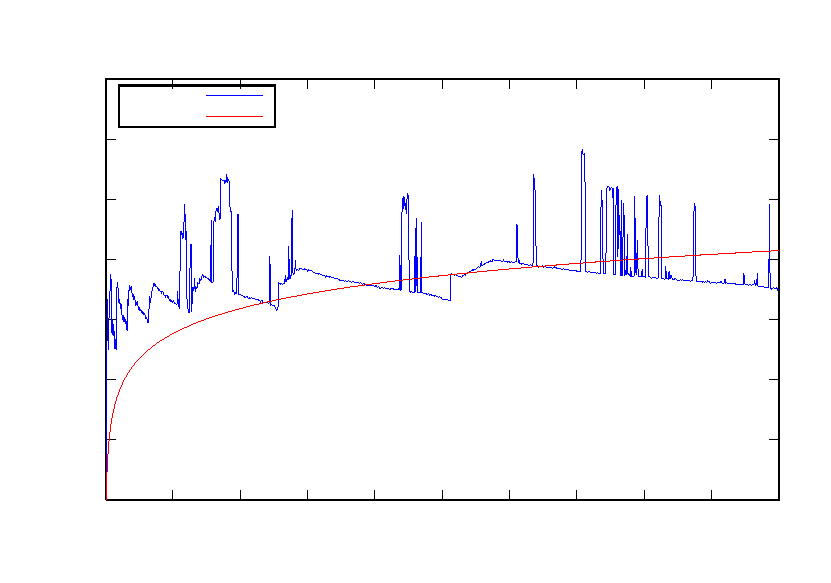
\includegraphics{problema2-mejor-caso-logn}}%
    \gplfronttext
  \end{picture}%
\endgroup

  \caption{Mejor caso ($log(n)$)}
\end{figure}

\begin{figure}[H]
  \centering
  % GNUPLOT: LaTeX picture with Postscript
\begingroup
  \makeatletter
  \providecommand\color[2][]{%
    \GenericError{(gnuplot) \space\space\space\@spaces}{%
      Package color not loaded in conjunction with
      terminal option `colourtext'%
    }{See the gnuplot documentation for explanation.%
    }{Either use 'blacktext' in gnuplot or load the package
      color.sty in LaTeX.}%
    \renewcommand\color[2][]{}%
  }%
  \providecommand\includegraphics[2][]{%
    \GenericError{(gnuplot) \space\space\space\@spaces}{%
      Package graphicx or graphics not loaded%
    }{See the gnuplot documentation for explanation.%
    }{The gnuplot epslatex terminal needs graphicx.sty or graphics.sty.}%
    \renewcommand\includegraphics[2][]{}%
  }%
  \providecommand\rotatebox[2]{#2}%
  \@ifundefined{ifGPcolor}{%
    \newif\ifGPcolor
    \GPcolorfalse
  }{}%
  \@ifundefined{ifGPblacktext}{%
    \newif\ifGPblacktext
    \GPblacktexttrue
  }{}%
  % define a \g@addto@macro without @ in the name:
  \let\gplgaddtomacro\g@addto@macro
  % define empty templates for all commands taking text:
  \gdef\gplbacktext{}%
  \gdef\gplfronttext{}%
  \makeatother
  \ifGPblacktext
    % no textcolor at all
    \def\colorrgb#1{}%
    \def\colorgray#1{}%
  \else
    % gray or color?
    \ifGPcolor
      \def\colorrgb#1{\color[rgb]{#1}}%
      \def\colorgray#1{\color[gray]{#1}}%
      \expandafter\def\csname LTw\endcsname{\color{white}}%
      \expandafter\def\csname LTb\endcsname{\color{black}}%
      \expandafter\def\csname LTa\endcsname{\color{black}}%
      \expandafter\def\csname LT0\endcsname{\color[rgb]{1,0,0}}%
      \expandafter\def\csname LT1\endcsname{\color[rgb]{0,1,0}}%
      \expandafter\def\csname LT2\endcsname{\color[rgb]{0,0,1}}%
      \expandafter\def\csname LT3\endcsname{\color[rgb]{1,0,1}}%
      \expandafter\def\csname LT4\endcsname{\color[rgb]{0,1,1}}%
      \expandafter\def\csname LT5\endcsname{\color[rgb]{1,1,0}}%
      \expandafter\def\csname LT6\endcsname{\color[rgb]{0,0,0}}%
      \expandafter\def\csname LT7\endcsname{\color[rgb]{1,0.3,0}}%
      \expandafter\def\csname LT8\endcsname{\color[rgb]{0.5,0.5,0.5}}%
    \else
      % gray
      \def\colorrgb#1{\color{black}}%
      \def\colorgray#1{\color[gray]{#1}}%
      \expandafter\def\csname LTw\endcsname{\color{white}}%
      \expandafter\def\csname LTb\endcsname{\color{black}}%
      \expandafter\def\csname LTa\endcsname{\color{black}}%
      \expandafter\def\csname LT0\endcsname{\color{black}}%
      \expandafter\def\csname LT1\endcsname{\color{black}}%
      \expandafter\def\csname LT2\endcsname{\color{black}}%
      \expandafter\def\csname LT3\endcsname{\color{black}}%
      \expandafter\def\csname LT4\endcsname{\color{black}}%
      \expandafter\def\csname LT5\endcsname{\color{black}}%
      \expandafter\def\csname LT6\endcsname{\color{black}}%
      \expandafter\def\csname LT7\endcsname{\color{black}}%
      \expandafter\def\csname LT8\endcsname{\color{black}}%
    \fi
  \fi
  \setlength{\unitlength}{0.0500bp}%
  \begin{picture}(9118.00,4320.00)%
    \gplgaddtomacro\gplbacktext{%
      \colorrgb{0.00,0.00,0.00}%
      \put(860,640){\makebox(0,0)[r]{\strut{}0}}%
      \colorrgb{0.00,0.00,0.00}%
      \put(860,1153){\makebox(0,0)[r]{\strut{}0.02}}%
      \colorrgb{0.00,0.00,0.00}%
      \put(860,1666){\makebox(0,0)[r]{\strut{}0.04}}%
      \colorrgb{0.00,0.00,0.00}%
      \put(860,2180){\makebox(0,0)[r]{\strut{}0.06}}%
      \colorrgb{0.00,0.00,0.00}%
      \put(860,2693){\makebox(0,0)[r]{\strut{}0.08}}%
      \colorrgb{0.00,0.00,0.00}%
      \put(860,3206){\makebox(0,0)[r]{\strut{}0.1}}%
      \colorrgb{0.00,0.00,0.00}%
      \put(860,3719){\makebox(0,0)[r]{\strut{}0.12}}%
      \colorrgb{0.00,0.00,0.00}%
      \put(972,440){\makebox(0,0){\strut{}0}}%
      \colorrgb{0.00,0.00,0.00}%
      \put(1751,440){\makebox(0,0){\strut{}100}}%
      \colorrgb{0.00,0.00,0.00}%
      \put(2529,440){\makebox(0,0){\strut{}200}}%
      \colorrgb{0.00,0.00,0.00}%
      \put(3308,440){\makebox(0,0){\strut{}300}}%
      \colorrgb{0.00,0.00,0.00}%
      \put(4086,440){\makebox(0,0){\strut{}400}}%
      \colorrgb{0.00,0.00,0.00}%
      \put(4865,440){\makebox(0,0){\strut{}500}}%
      \colorrgb{0.00,0.00,0.00}%
      \put(5643,440){\makebox(0,0){\strut{}600}}%
      \colorrgb{0.00,0.00,0.00}%
      \put(6422,440){\makebox(0,0){\strut{}700}}%
      \colorrgb{0.00,0.00,0.00}%
      \put(7200,440){\makebox(0,0){\strut{}800}}%
      \colorrgb{0.00,0.00,0.00}%
      \put(7979,440){\makebox(0,0){\strut{}900}}%
      \colorrgb{0.00,0.00,0.00}%
      \put(8757,440){\makebox(0,0){\strut{}1000}}%
      \colorrgb{0.00,0.00,0.00}%
      \put(160,2179){\rotatebox{90}{\makebox(0,0){\strut{}Tiempo [$mS$]}}}%
      \colorrgb{0.00,0.00,0.00}%
      \put(4868,140){\makebox(0,0){\strut{}$n$ (tama\~no del problema)}}%
      \csname LTb\endcsname%
      \put(4868,4019){\makebox(0,0){\strut{}Tiempo de ejecuci\'on dividido por $log(n)$}}%
    }%
    \gplgaddtomacro\gplfronttext{%
      \csname LTb\endcsname%
      \put(2660,3556){\makebox(0,0)[r]{\strut{}$T(n) / log(n)$}}%
      \csname LTb\endcsname%
      \put(2660,3356){\makebox(0,0)[r]{\strut{}$O(n)$}}%
    }%
    \gplbacktext
    \put(0,0){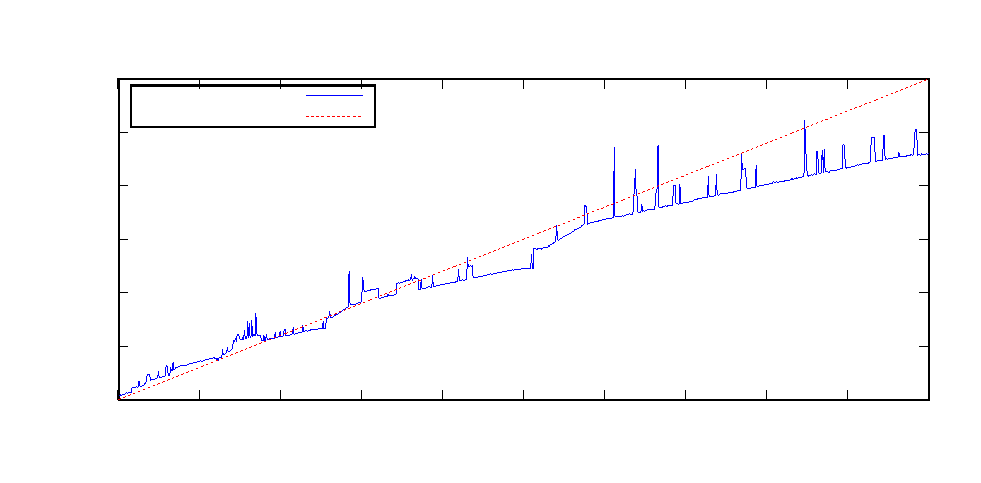
\includegraphics{problema2-mejor-caso-n}}%
    \gplfronttext
  \end{picture}%
\endgroup

  \caption{Mejor caso ($n$)}
\end{figure}


\subsubsection{Instancias aleatorias}

\begin{figure}[H]
  \centering
  % GNUPLOT: LaTeX picture with Postscript
\begingroup
  \makeatletter
  \providecommand\color[2][]{%
    \GenericError{(gnuplot) \space\space\space\@spaces}{%
      Package color not loaded in conjunction with
      terminal option `colourtext'%
    }{See the gnuplot documentation for explanation.%
    }{Either use 'blacktext' in gnuplot or load the package
      color.sty in LaTeX.}%
    \renewcommand\color[2][]{}%
  }%
  \providecommand\includegraphics[2][]{%
    \GenericError{(gnuplot) \space\space\space\@spaces}{%
      Package graphicx or graphics not loaded%
    }{See the gnuplot documentation for explanation.%
    }{The gnuplot epslatex terminal needs graphicx.sty or graphics.sty.}%
    \renewcommand\includegraphics[2][]{}%
  }%
  \providecommand\rotatebox[2]{#2}%
  \@ifundefined{ifGPcolor}{%
    \newif\ifGPcolor
    \GPcolorfalse
  }{}%
  \@ifundefined{ifGPblacktext}{%
    \newif\ifGPblacktext
    \GPblacktexttrue
  }{}%
  % define a \g@addto@macro without @ in the name:
  \let\gplgaddtomacro\g@addto@macro
  % define empty templates for all commands taking text:
  \gdef\gplbacktext{}%
  \gdef\gplfronttext{}%
  \makeatother
  \ifGPblacktext
    % no textcolor at all
    \def\colorrgb#1{}%
    \def\colorgray#1{}%
  \else
    % gray or color?
    \ifGPcolor
      \def\colorrgb#1{\color[rgb]{#1}}%
      \def\colorgray#1{\color[gray]{#1}}%
      \expandafter\def\csname LTw\endcsname{\color{white}}%
      \expandafter\def\csname LTb\endcsname{\color{black}}%
      \expandafter\def\csname LTa\endcsname{\color{black}}%
      \expandafter\def\csname LT0\endcsname{\color[rgb]{1,0,0}}%
      \expandafter\def\csname LT1\endcsname{\color[rgb]{0,1,0}}%
      \expandafter\def\csname LT2\endcsname{\color[rgb]{0,0,1}}%
      \expandafter\def\csname LT3\endcsname{\color[rgb]{1,0,1}}%
      \expandafter\def\csname LT4\endcsname{\color[rgb]{0,1,1}}%
      \expandafter\def\csname LT5\endcsname{\color[rgb]{1,1,0}}%
      \expandafter\def\csname LT6\endcsname{\color[rgb]{0,0,0}}%
      \expandafter\def\csname LT7\endcsname{\color[rgb]{1,0.3,0}}%
      \expandafter\def\csname LT8\endcsname{\color[rgb]{0.5,0.5,0.5}}%
    \else
      % gray
      \def\colorrgb#1{\color{black}}%
      \def\colorgray#1{\color[gray]{#1}}%
      \expandafter\def\csname LTw\endcsname{\color{white}}%
      \expandafter\def\csname LTb\endcsname{\color{black}}%
      \expandafter\def\csname LTa\endcsname{\color{black}}%
      \expandafter\def\csname LT0\endcsname{\color{black}}%
      \expandafter\def\csname LT1\endcsname{\color{black}}%
      \expandafter\def\csname LT2\endcsname{\color{black}}%
      \expandafter\def\csname LT3\endcsname{\color{black}}%
      \expandafter\def\csname LT4\endcsname{\color{black}}%
      \expandafter\def\csname LT5\endcsname{\color{black}}%
      \expandafter\def\csname LT6\endcsname{\color{black}}%
      \expandafter\def\csname LT7\endcsname{\color{black}}%
      \expandafter\def\csname LT8\endcsname{\color{black}}%
    \fi
  \fi
  \setlength{\unitlength}{0.0500bp}%
  \begin{picture}(7678.00,5280.00)%
    \gplgaddtomacro\gplbacktext{%
      \colorrgb{0.00,0.00,0.00}%
      \put(740,640){\makebox(0,0)[r]{\strut{}0}}%
      \colorrgb{0.00,0.00,0.00}%
      \put(740,1217){\makebox(0,0)[r]{\strut{}0.2}}%
      \colorrgb{0.00,0.00,0.00}%
      \put(740,1794){\makebox(0,0)[r]{\strut{}0.4}}%
      \colorrgb{0.00,0.00,0.00}%
      \put(740,2371){\makebox(0,0)[r]{\strut{}0.6}}%
      \colorrgb{0.00,0.00,0.00}%
      \put(740,2948){\makebox(0,0)[r]{\strut{}0.8}}%
      \colorrgb{0.00,0.00,0.00}%
      \put(740,3525){\makebox(0,0)[r]{\strut{}1}}%
      \colorrgb{0.00,0.00,0.00}%
      \put(740,4102){\makebox(0,0)[r]{\strut{}1.2}}%
      \colorrgb{0.00,0.00,0.00}%
      \put(740,4679){\makebox(0,0)[r]{\strut{}1.4}}%
      \colorrgb{0.00,0.00,0.00}%
      \put(860,440){\makebox(0,0){\strut{}100}}%
      \colorrgb{0.00,0.00,0.00}%
      \put(1666,440){\makebox(0,0){\strut{}200}}%
      \colorrgb{0.00,0.00,0.00}%
      \put(2472,440){\makebox(0,0){\strut{}300}}%
      \colorrgb{0.00,0.00,0.00}%
      \put(3278,440){\makebox(0,0){\strut{}400}}%
      \colorrgb{0.00,0.00,0.00}%
      \put(4084,440){\makebox(0,0){\strut{}500}}%
      \colorrgb{0.00,0.00,0.00}%
      \put(4891,440){\makebox(0,0){\strut{}600}}%
      \colorrgb{0.00,0.00,0.00}%
      \put(5697,440){\makebox(0,0){\strut{}700}}%
      \colorrgb{0.00,0.00,0.00}%
      \put(6503,440){\makebox(0,0){\strut{}800}}%
      \colorrgb{0.00,0.00,0.00}%
      \put(7309,440){\makebox(0,0){\strut{}900}}%
      \colorrgb{0.00,0.00,0.00}%
      \put(160,2659){\rotatebox{90}{\makebox(0,0){\strut{}Tiempo de ejecuci\'on [$mS$]}}}%
      \colorrgb{0.00,0.00,0.00}%
      \put(4088,140){\makebox(0,0){\strut{}$n$ (tama\~no del problema)}}%
      \csname LTb\endcsname%
      \put(4088,4979){\makebox(0,0){\strut{}Instancias aleatorias}}%
    }%
    \gplgaddtomacro\gplfronttext{%
      \csname LTb\endcsname%
      \put(2180,4516){\makebox(0,0)[r]{\strut{}$t_n$}}%
      \csname LTb\endcsname%
      \put(2180,4316){\makebox(0,0)[r]{\strut{}$n * log(n)$}}%
    }%
    \gplbacktext
    \put(0,0){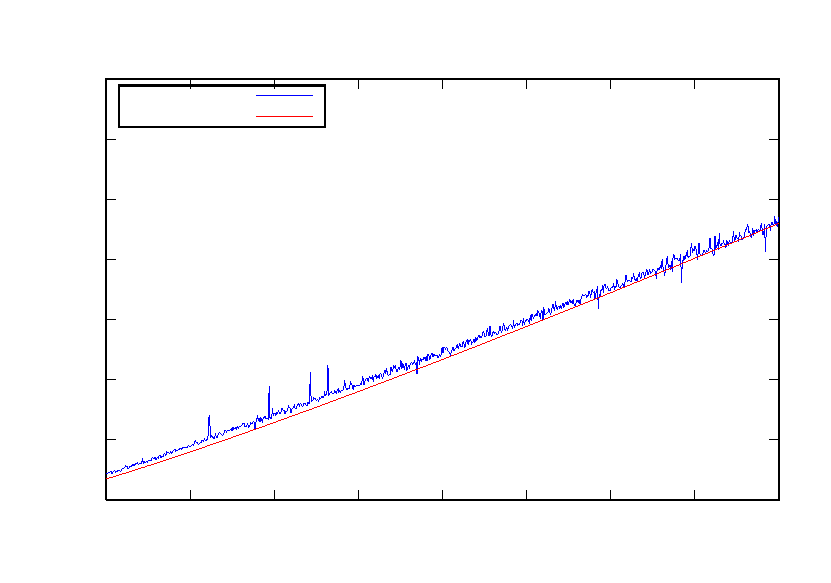
\includegraphics{problema2-instancias-aleatorias}}%
    \gplfronttext
  \end{picture}%
\endgroup

  \caption{Instancias aleatorias}
\end{figure}

\begin{figure}[H]
  \centering
  % GNUPLOT: LaTeX picture with Postscript
\begingroup
  \makeatletter
  \providecommand\color[2][]{%
    \GenericError{(gnuplot) \space\space\space\@spaces}{%
      Package color not loaded in conjunction with
      terminal option `colourtext'%
    }{See the gnuplot documentation for explanation.%
    }{Either use 'blacktext' in gnuplot or load the package
      color.sty in LaTeX.}%
    \renewcommand\color[2][]{}%
  }%
  \providecommand\includegraphics[2][]{%
    \GenericError{(gnuplot) \space\space\space\@spaces}{%
      Package graphicx or graphics not loaded%
    }{See the gnuplot documentation for explanation.%
    }{The gnuplot epslatex terminal needs graphicx.sty or graphics.sty.}%
    \renewcommand\includegraphics[2][]{}%
  }%
  \providecommand\rotatebox[2]{#2}%
  \@ifundefined{ifGPcolor}{%
    \newif\ifGPcolor
    \GPcolorfalse
  }{}%
  \@ifundefined{ifGPblacktext}{%
    \newif\ifGPblacktext
    \GPblacktexttrue
  }{}%
  % define a \g@addto@macro without @ in the name:
  \let\gplgaddtomacro\g@addto@macro
  % define empty templates for all commands taking text:
  \gdef\gplbacktext{}%
  \gdef\gplfronttext{}%
  \makeatother
  \ifGPblacktext
    % no textcolor at all
    \def\colorrgb#1{}%
    \def\colorgray#1{}%
  \else
    % gray or color?
    \ifGPcolor
      \def\colorrgb#1{\color[rgb]{#1}}%
      \def\colorgray#1{\color[gray]{#1}}%
      \expandafter\def\csname LTw\endcsname{\color{white}}%
      \expandafter\def\csname LTb\endcsname{\color{black}}%
      \expandafter\def\csname LTa\endcsname{\color{black}}%
      \expandafter\def\csname LT0\endcsname{\color[rgb]{1,0,0}}%
      \expandafter\def\csname LT1\endcsname{\color[rgb]{0,1,0}}%
      \expandafter\def\csname LT2\endcsname{\color[rgb]{0,0,1}}%
      \expandafter\def\csname LT3\endcsname{\color[rgb]{1,0,1}}%
      \expandafter\def\csname LT4\endcsname{\color[rgb]{0,1,1}}%
      \expandafter\def\csname LT5\endcsname{\color[rgb]{1,1,0}}%
      \expandafter\def\csname LT6\endcsname{\color[rgb]{0,0,0}}%
      \expandafter\def\csname LT7\endcsname{\color[rgb]{1,0.3,0}}%
      \expandafter\def\csname LT8\endcsname{\color[rgb]{0.5,0.5,0.5}}%
    \else
      % gray
      \def\colorrgb#1{\color{black}}%
      \def\colorgray#1{\color[gray]{#1}}%
      \expandafter\def\csname LTw\endcsname{\color{white}}%
      \expandafter\def\csname LTb\endcsname{\color{black}}%
      \expandafter\def\csname LTa\endcsname{\color{black}}%
      \expandafter\def\csname LT0\endcsname{\color{black}}%
      \expandafter\def\csname LT1\endcsname{\color{black}}%
      \expandafter\def\csname LT2\endcsname{\color{black}}%
      \expandafter\def\csname LT3\endcsname{\color{black}}%
      \expandafter\def\csname LT4\endcsname{\color{black}}%
      \expandafter\def\csname LT5\endcsname{\color{black}}%
      \expandafter\def\csname LT6\endcsname{\color{black}}%
      \expandafter\def\csname LT7\endcsname{\color{black}}%
      \expandafter\def\csname LT8\endcsname{\color{black}}%
    \fi
  \fi
  \setlength{\unitlength}{0.0500bp}%
  \begin{picture}(9118.00,4320.00)%
    \gplgaddtomacro\gplbacktext{%
      \colorrgb{0.00,0.00,0.00}%
      \put(740,640){\makebox(0,0)[r]{\strut{}0}}%
      \colorrgb{0.00,0.00,0.00}%
      \put(740,1080){\makebox(0,0)[r]{\strut{}0.2}}%
      \colorrgb{0.00,0.00,0.00}%
      \put(740,1520){\makebox(0,0)[r]{\strut{}0.4}}%
      \colorrgb{0.00,0.00,0.00}%
      \put(740,1960){\makebox(0,0)[r]{\strut{}0.6}}%
      \colorrgb{0.00,0.00,0.00}%
      \put(740,2399){\makebox(0,0)[r]{\strut{}0.8}}%
      \colorrgb{0.00,0.00,0.00}%
      \put(740,2839){\makebox(0,0)[r]{\strut{}1}}%
      \colorrgb{0.00,0.00,0.00}%
      \put(740,3279){\makebox(0,0)[r]{\strut{}1.2}}%
      \colorrgb{0.00,0.00,0.00}%
      \put(740,3719){\makebox(0,0)[r]{\strut{}1.4}}%
      \colorrgb{0.00,0.00,0.00}%
      \put(852,440){\makebox(0,0){\strut{}0}}%
      \colorrgb{0.00,0.00,0.00}%
      \put(1643,440){\makebox(0,0){\strut{}100}}%
      \colorrgb{0.00,0.00,0.00}%
      \put(2433,440){\makebox(0,0){\strut{}200}}%
      \colorrgb{0.00,0.00,0.00}%
      \put(3224,440){\makebox(0,0){\strut{}300}}%
      \colorrgb{0.00,0.00,0.00}%
      \put(4014,440){\makebox(0,0){\strut{}400}}%
      \colorrgb{0.00,0.00,0.00}%
      \put(4805,440){\makebox(0,0){\strut{}500}}%
      \colorrgb{0.00,0.00,0.00}%
      \put(5595,440){\makebox(0,0){\strut{}600}}%
      \colorrgb{0.00,0.00,0.00}%
      \put(6386,440){\makebox(0,0){\strut{}700}}%
      \colorrgb{0.00,0.00,0.00}%
      \put(7176,440){\makebox(0,0){\strut{}800}}%
      \colorrgb{0.00,0.00,0.00}%
      \put(7967,440){\makebox(0,0){\strut{}900}}%
      \colorrgb{0.00,0.00,0.00}%
      \put(8757,440){\makebox(0,0){\strut{}1000}}%
      \colorrgb{0.00,0.00,0.00}%
      \put(160,2179){\rotatebox{90}{\makebox(0,0){\strut{}Tiempo [$\mu S$]}}}%
      \colorrgb{0.00,0.00,0.00}%
      \put(4808,140){\makebox(0,0){\strut{}$n$ (tama\~no del problema)}}%
      \csname LTb\endcsname%
      \put(4808,4019){\makebox(0,0){\strut{}Tiempo de ejecuci\'on dividido por $n$}}%
    }%
    \gplgaddtomacro\gplfronttext{%
      \csname LTb\endcsname%
      \put(2060,3556){\makebox(0,0)[r]{\strut{}$T(n) / n$}}%
      \csname LTb\endcsname%
      \put(2060,3356){\makebox(0,0)[r]{\strut{}$O(log(n))$}}%
    }%
    \gplbacktext
    \put(0,0){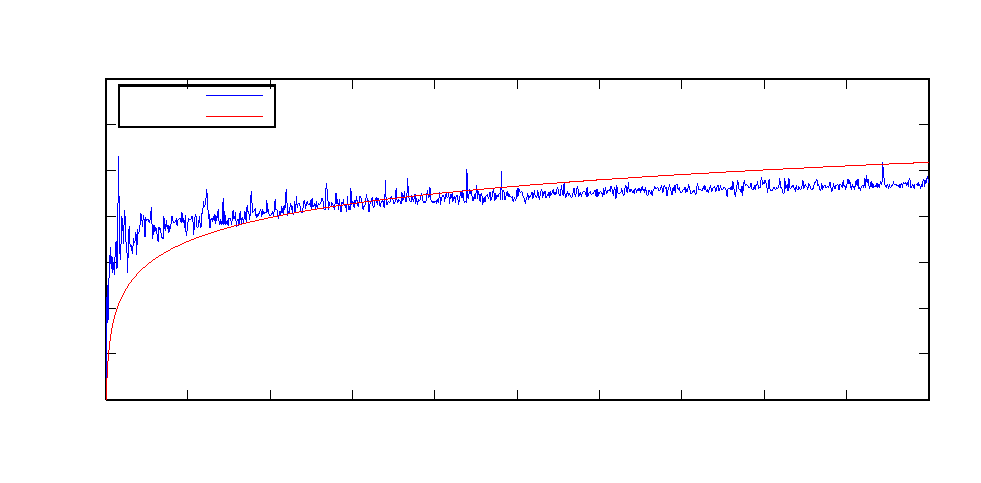
\includegraphics{problema2-instancias-aleatorias-logn}}%
    \gplfronttext
  \end{picture}%
\endgroup

  \caption{Instancias aleatorias ($log(n)$)}
\end{figure}

\begin{figure}[H]
  \centering
  % GNUPLOT: LaTeX picture with Postscript
\begingroup
  \makeatletter
  \providecommand\color[2][]{%
    \GenericError{(gnuplot) \space\space\space\@spaces}{%
      Package color not loaded in conjunction with
      terminal option `colourtext'%
    }{See the gnuplot documentation for explanation.%
    }{Either use 'blacktext' in gnuplot or load the package
      color.sty in LaTeX.}%
    \renewcommand\color[2][]{}%
  }%
  \providecommand\includegraphics[2][]{%
    \GenericError{(gnuplot) \space\space\space\@spaces}{%
      Package graphicx or graphics not loaded%
    }{See the gnuplot documentation for explanation.%
    }{The gnuplot epslatex terminal needs graphicx.sty or graphics.sty.}%
    \renewcommand\includegraphics[2][]{}%
  }%
  \providecommand\rotatebox[2]{#2}%
  \@ifundefined{ifGPcolor}{%
    \newif\ifGPcolor
    \GPcolorfalse
  }{}%
  \@ifundefined{ifGPblacktext}{%
    \newif\ifGPblacktext
    \GPblacktexttrue
  }{}%
  % define a \g@addto@macro without @ in the name:
  \let\gplgaddtomacro\g@addto@macro
  % define empty templates for all commands taking text:
  \gdef\gplbacktext{}%
  \gdef\gplfronttext{}%
  \makeatother
  \ifGPblacktext
    % no textcolor at all
    \def\colorrgb#1{}%
    \def\colorgray#1{}%
  \else
    % gray or color?
    \ifGPcolor
      \def\colorrgb#1{\color[rgb]{#1}}%
      \def\colorgray#1{\color[gray]{#1}}%
      \expandafter\def\csname LTw\endcsname{\color{white}}%
      \expandafter\def\csname LTb\endcsname{\color{black}}%
      \expandafter\def\csname LTa\endcsname{\color{black}}%
      \expandafter\def\csname LT0\endcsname{\color[rgb]{1,0,0}}%
      \expandafter\def\csname LT1\endcsname{\color[rgb]{0,1,0}}%
      \expandafter\def\csname LT2\endcsname{\color[rgb]{0,0,1}}%
      \expandafter\def\csname LT3\endcsname{\color[rgb]{1,0,1}}%
      \expandafter\def\csname LT4\endcsname{\color[rgb]{0,1,1}}%
      \expandafter\def\csname LT5\endcsname{\color[rgb]{1,1,0}}%
      \expandafter\def\csname LT6\endcsname{\color[rgb]{0,0,0}}%
      \expandafter\def\csname LT7\endcsname{\color[rgb]{1,0.3,0}}%
      \expandafter\def\csname LT8\endcsname{\color[rgb]{0.5,0.5,0.5}}%
    \else
      % gray
      \def\colorrgb#1{\color{black}}%
      \def\colorgray#1{\color[gray]{#1}}%
      \expandafter\def\csname LTw\endcsname{\color{white}}%
      \expandafter\def\csname LTb\endcsname{\color{black}}%
      \expandafter\def\csname LTa\endcsname{\color{black}}%
      \expandafter\def\csname LT0\endcsname{\color{black}}%
      \expandafter\def\csname LT1\endcsname{\color{black}}%
      \expandafter\def\csname LT2\endcsname{\color{black}}%
      \expandafter\def\csname LT3\endcsname{\color{black}}%
      \expandafter\def\csname LT4\endcsname{\color{black}}%
      \expandafter\def\csname LT5\endcsname{\color{black}}%
      \expandafter\def\csname LT6\endcsname{\color{black}}%
      \expandafter\def\csname LT7\endcsname{\color{black}}%
      \expandafter\def\csname LT8\endcsname{\color{black}}%
    \fi
  \fi
  \setlength{\unitlength}{0.0500bp}%
  \begin{picture}(9118.00,4320.00)%
    \gplgaddtomacro\gplbacktext{%
      \colorrgb{0.00,0.00,0.00}%
      \put(860,640){\makebox(0,0)[r]{\strut{}0}}%
      \colorrgb{0.00,0.00,0.00}%
      \put(860,1410){\makebox(0,0)[r]{\strut{}0.05}}%
      \colorrgb{0.00,0.00,0.00}%
      \put(860,2180){\makebox(0,0)[r]{\strut{}0.1}}%
      \colorrgb{0.00,0.00,0.00}%
      \put(860,2949){\makebox(0,0)[r]{\strut{}0.15}}%
      \colorrgb{0.00,0.00,0.00}%
      \put(860,3719){\makebox(0,0)[r]{\strut{}0.2}}%
      \colorrgb{0.00,0.00,0.00}%
      \put(972,440){\makebox(0,0){\strut{}0}}%
      \colorrgb{0.00,0.00,0.00}%
      \put(1751,440){\makebox(0,0){\strut{}100}}%
      \colorrgb{0.00,0.00,0.00}%
      \put(2529,440){\makebox(0,0){\strut{}200}}%
      \colorrgb{0.00,0.00,0.00}%
      \put(3308,440){\makebox(0,0){\strut{}300}}%
      \colorrgb{0.00,0.00,0.00}%
      \put(4086,440){\makebox(0,0){\strut{}400}}%
      \colorrgb{0.00,0.00,0.00}%
      \put(4865,440){\makebox(0,0){\strut{}500}}%
      \colorrgb{0.00,0.00,0.00}%
      \put(5643,440){\makebox(0,0){\strut{}600}}%
      \colorrgb{0.00,0.00,0.00}%
      \put(6422,440){\makebox(0,0){\strut{}700}}%
      \colorrgb{0.00,0.00,0.00}%
      \put(7200,440){\makebox(0,0){\strut{}800}}%
      \colorrgb{0.00,0.00,0.00}%
      \put(7979,440){\makebox(0,0){\strut{}900}}%
      \colorrgb{0.00,0.00,0.00}%
      \put(8757,440){\makebox(0,0){\strut{}1000}}%
      \colorrgb{0.00,0.00,0.00}%
      \put(160,2179){\rotatebox{90}{\makebox(0,0){\strut{}Tiempo [$mS$]}}}%
      \colorrgb{0.00,0.00,0.00}%
      \put(4868,140){\makebox(0,0){\strut{}$n$ (tama\~no del problema)}}%
      \csname LTb\endcsname%
      \put(4868,4019){\makebox(0,0){\strut{}Tiempo de ejecuci\'on dividido por $log(n)$}}%
    }%
    \gplgaddtomacro\gplfronttext{%
      \csname LTb\endcsname%
      \put(2420,3556){\makebox(0,0)[r]{\strut{}$t_n / log(n)$}}%
      \csname LTb\endcsname%
      \put(2420,3356){\makebox(0,0)[r]{\strut{}$n$}}%
    }%
    \gplbacktext
    \put(0,0){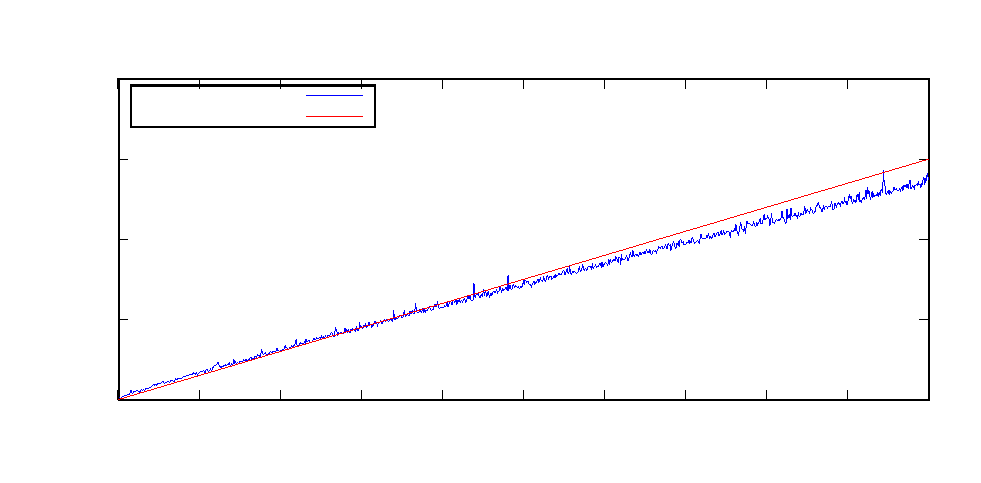
\includegraphics{problema2-instancias-aleatorias-n}}%
    \gplfronttext
  \end{picture}%
\endgroup

  \caption{Instancias aleatorias ($n$)}
\end{figure}



%%%%%%%%%%%%%%%%%%%%%%%%%%%%%%%%%%%%%%%%%%%%%%%%%%%%%%%%%%%%%%%%%%%%%%%%%%%%%%%
%% Problema 3: Una noche en el museo                                         %%
%%%%%%%%%%%%%%%%%%%%%%%%%%%%%%%%%%%%%%%%%%%%%%%%%%%%%%%%%%%%%%%%%%%%%%%%%%%%%%%


\newpage

\section{Problema 3: Una noche en el museo}
Se desea instalar un sistema de detección de movimientos basado en sensores láser, para esto cada piso del museo fue modelado por una grilla de $n$ $x$ $m$ casillas.

Existen dos tipos de sensores, bidireccionales (emiten señales hacia la izquierda y la derecha o bien hacia arriba y abajo) y cuatridireccionales (emiten señales en las 4 direcciones), de \$4000 y \$6000 respectivamente y 3 tipos de casilla, vacía, importante y pared.

Dado un piso se debe cumplir:

\begin{itemize}
\item las casillas libres deben quedar cubiertas por al menos un sensor.
\item las casilla importantes deben ser cubiertas por dos sensores.
\item no se puede ubicar un sensor de forma tal que alguna de sus señales impacten contra otro dispositivo.
\item no se puede instalar más de un dispositivo en una misma casilla libre.
\item en caso de haber solución, la misma debrá minimizar la cantidad de dinero invertido en sensores.
\end{itemize}

Se pide realizar el algoritmo mediante la técnica de Backtracking.

Ejemplo:
\begin{figure}[H]
  \centering
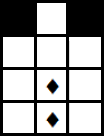
\includegraphics[width=0.20\textwidth]{ejemplo_problema3/grilla.png}
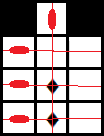
\includegraphics[width=0.20\textwidth]{ejemplo_problema3/grilla-sol16000.png}
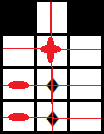
\includegraphics[width=0.20\textwidth]{ejemplo_problema3/grilla-sol14000.png}
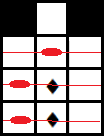
\includegraphics[width=0.20\textwidth]{ejemplo_problema3/grillaSinSol.png}
  \caption{Instacia del problema, dos soluciones distintas con un costo de \$14.000 y \$16.000 respectivamente y una solución no válida} 
  \label{fig:1}
\end{figure}


\subsubsection{Peor caso}

\begin{figure}[H]
  \centering
  % GNUPLOT: LaTeX picture with Postscript
\begingroup
  \makeatletter
  \providecommand\color[2][]{%
    \GenericError{(gnuplot) \space\space\space\@spaces}{%
      Package color not loaded in conjunction with
      terminal option `colourtext'%
    }{See the gnuplot documentation for explanation.%
    }{Either use 'blacktext' in gnuplot or load the package
      color.sty in LaTeX.}%
    \renewcommand\color[2][]{}%
  }%
  \providecommand\includegraphics[2][]{%
    \GenericError{(gnuplot) \space\space\space\@spaces}{%
      Package graphicx or graphics not loaded%
    }{See the gnuplot documentation for explanation.%
    }{The gnuplot epslatex terminal needs graphicx.sty or graphics.sty.}%
    \renewcommand\includegraphics[2][]{}%
  }%
  \providecommand\rotatebox[2]{#2}%
  \@ifundefined{ifGPcolor}{%
    \newif\ifGPcolor
    \GPcolorfalse
  }{}%
  \@ifundefined{ifGPblacktext}{%
    \newif\ifGPblacktext
    \GPblacktexttrue
  }{}%
  % define a \g@addto@macro without @ in the name:
  \let\gplgaddtomacro\g@addto@macro
  % define empty templates for all commands taking text:
  \gdef\gplbacktext{}%
  \gdef\gplfronttext{}%
  \makeatother
  \ifGPblacktext
    % no textcolor at all
    \def\colorrgb#1{}%
    \def\colorgray#1{}%
  \else
    % gray or color?
    \ifGPcolor
      \def\colorrgb#1{\color[rgb]{#1}}%
      \def\colorgray#1{\color[gray]{#1}}%
      \expandafter\def\csname LTw\endcsname{\color{white}}%
      \expandafter\def\csname LTb\endcsname{\color{black}}%
      \expandafter\def\csname LTa\endcsname{\color{black}}%
      \expandafter\def\csname LT0\endcsname{\color[rgb]{1,0,0}}%
      \expandafter\def\csname LT1\endcsname{\color[rgb]{0,1,0}}%
      \expandafter\def\csname LT2\endcsname{\color[rgb]{0,0,1}}%
      \expandafter\def\csname LT3\endcsname{\color[rgb]{1,0,1}}%
      \expandafter\def\csname LT4\endcsname{\color[rgb]{0,1,1}}%
      \expandafter\def\csname LT5\endcsname{\color[rgb]{1,1,0}}%
      \expandafter\def\csname LT6\endcsname{\color[rgb]{0,0,0}}%
      \expandafter\def\csname LT7\endcsname{\color[rgb]{1,0.3,0}}%
      \expandafter\def\csname LT8\endcsname{\color[rgb]{0.5,0.5,0.5}}%
    \else
      % gray
      \def\colorrgb#1{\color{black}}%
      \def\colorgray#1{\color[gray]{#1}}%
      \expandafter\def\csname LTw\endcsname{\color{white}}%
      \expandafter\def\csname LTb\endcsname{\color{black}}%
      \expandafter\def\csname LTa\endcsname{\color{black}}%
      \expandafter\def\csname LT0\endcsname{\color{black}}%
      \expandafter\def\csname LT1\endcsname{\color{black}}%
      \expandafter\def\csname LT2\endcsname{\color{black}}%
      \expandafter\def\csname LT3\endcsname{\color{black}}%
      \expandafter\def\csname LT4\endcsname{\color{black}}%
      \expandafter\def\csname LT5\endcsname{\color{black}}%
      \expandafter\def\csname LT6\endcsname{\color{black}}%
      \expandafter\def\csname LT7\endcsname{\color{black}}%
      \expandafter\def\csname LT8\endcsname{\color{black}}%
    \fi
  \fi
  \setlength{\unitlength}{0.0500bp}%
  \begin{picture}(9118.00,4320.00)%
    \gplgaddtomacro\gplbacktext{%
      \colorrgb{0.00,0.00,0.00}%
      \put(860,640){\makebox(0,0)[r]{\strut{}$10^{-2}$}}%
      \colorrgb{0.00,0.00,0.00}%
      \put(860,1256){\makebox(0,0)[r]{\strut{}$10^{-1}$}}%
      \colorrgb{0.00,0.00,0.00}%
      \put(860,1872){\makebox(0,0)[r]{\strut{}$10^{0}$}}%
      \colorrgb{0.00,0.00,0.00}%
      \put(860,2487){\makebox(0,0)[r]{\strut{}$10^{1}$}}%
      \colorrgb{0.00,0.00,0.00}%
      \put(860,3103){\makebox(0,0)[r]{\strut{}$10^{2}$}}%
      \colorrgb{0.00,0.00,0.00}%
      \put(860,3719){\makebox(0,0)[r]{\strut{}$10^{3}$}}%
      \colorrgb{0.00,0.00,0.00}%
      \put(980,440){\makebox(0,0){\strut{}1x1,}}%
      \colorrgb{0.00,0.00,0.00}%
      \put(3572,440){\makebox(0,0){\strut{}2x2,}}%
      \colorrgb{0.00,0.00,0.00}%
      \put(6165,440){\makebox(0,0){\strut{}4x3,}}%
      \colorrgb{0.00,0.00,0.00}%
      \put(8757,440){\makebox(0,0){\strut{}5x5,}}%
      \colorrgb{0.00,0.00,0.00}%
      \put(160,2179){\rotatebox{90}{\makebox(0,0){\strut{}Tiempo de ejecuci\'on [$mS$]}}}%
      \colorrgb{0.00,0.00,0.00}%
      \put(4868,140){\makebox(0,0){\strut{}$n$ (tama\~no del problema)}}%
      \csname LTb\endcsname%
      \put(4868,4019){\makebox(0,0){\strut{}Peor caso}}%
    }%
    \gplgaddtomacro\gplfronttext{%
      \csname LTb\endcsname%
      \put(1340,3556){\makebox(0,0)[r]{\strut{}$t_n$}}%
    }%
    \gplbacktext
    \put(0,0){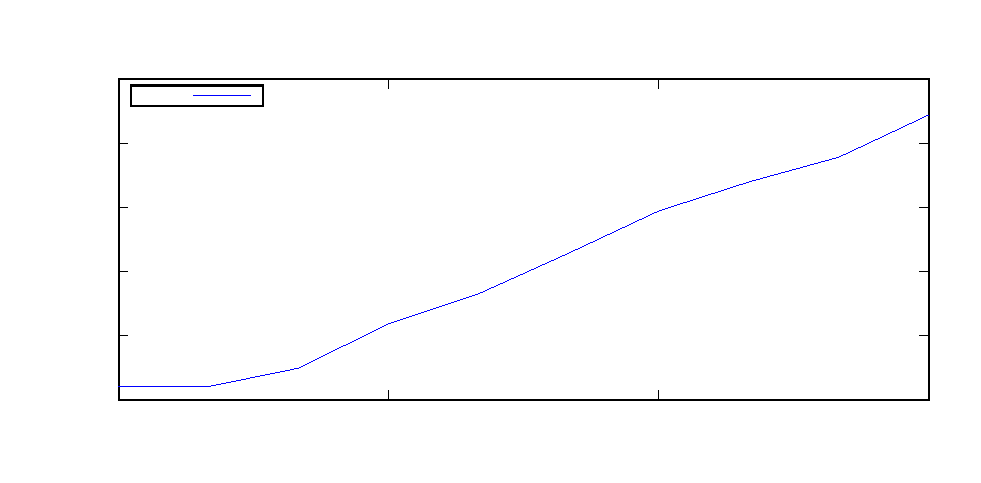
\includegraphics{problema3-peor-caso}}%
    \gplfronttext
  \end{picture}%
\endgroup

  \caption{Peor caso}
\end{figure}


\subsubsection{Mejor caso}

\begin{figure}[H]
  \centering
  % GNUPLOT: LaTeX picture with Postscript
\begingroup
  \makeatletter
  \providecommand\color[2][]{%
    \GenericError{(gnuplot) \space\space\space\@spaces}{%
      Package color not loaded in conjunction with
      terminal option `colourtext'%
    }{See the gnuplot documentation for explanation.%
    }{Either use 'blacktext' in gnuplot or load the package
      color.sty in LaTeX.}%
    \renewcommand\color[2][]{}%
  }%
  \providecommand\includegraphics[2][]{%
    \GenericError{(gnuplot) \space\space\space\@spaces}{%
      Package graphicx or graphics not loaded%
    }{See the gnuplot documentation for explanation.%
    }{The gnuplot epslatex terminal needs graphicx.sty or graphics.sty.}%
    \renewcommand\includegraphics[2][]{}%
  }%
  \providecommand\rotatebox[2]{#2}%
  \@ifundefined{ifGPcolor}{%
    \newif\ifGPcolor
    \GPcolorfalse
  }{}%
  \@ifundefined{ifGPblacktext}{%
    \newif\ifGPblacktext
    \GPblacktexttrue
  }{}%
  % define a \g@addto@macro without @ in the name:
  \let\gplgaddtomacro\g@addto@macro
  % define empty templates for all commands taking text:
  \gdef\gplbacktext{}%
  \gdef\gplfronttext{}%
  \makeatother
  \ifGPblacktext
    % no textcolor at all
    \def\colorrgb#1{}%
    \def\colorgray#1{}%
  \else
    % gray or color?
    \ifGPcolor
      \def\colorrgb#1{\color[rgb]{#1}}%
      \def\colorgray#1{\color[gray]{#1}}%
      \expandafter\def\csname LTw\endcsname{\color{white}}%
      \expandafter\def\csname LTb\endcsname{\color{black}}%
      \expandafter\def\csname LTa\endcsname{\color{black}}%
      \expandafter\def\csname LT0\endcsname{\color[rgb]{1,0,0}}%
      \expandafter\def\csname LT1\endcsname{\color[rgb]{0,1,0}}%
      \expandafter\def\csname LT2\endcsname{\color[rgb]{0,0,1}}%
      \expandafter\def\csname LT3\endcsname{\color[rgb]{1,0,1}}%
      \expandafter\def\csname LT4\endcsname{\color[rgb]{0,1,1}}%
      \expandafter\def\csname LT5\endcsname{\color[rgb]{1,1,0}}%
      \expandafter\def\csname LT6\endcsname{\color[rgb]{0,0,0}}%
      \expandafter\def\csname LT7\endcsname{\color[rgb]{1,0.3,0}}%
      \expandafter\def\csname LT8\endcsname{\color[rgb]{0.5,0.5,0.5}}%
    \else
      % gray
      \def\colorrgb#1{\color{black}}%
      \def\colorgray#1{\color[gray]{#1}}%
      \expandafter\def\csname LTw\endcsname{\color{white}}%
      \expandafter\def\csname LTb\endcsname{\color{black}}%
      \expandafter\def\csname LTa\endcsname{\color{black}}%
      \expandafter\def\csname LT0\endcsname{\color{black}}%
      \expandafter\def\csname LT1\endcsname{\color{black}}%
      \expandafter\def\csname LT2\endcsname{\color{black}}%
      \expandafter\def\csname LT3\endcsname{\color{black}}%
      \expandafter\def\csname LT4\endcsname{\color{black}}%
      \expandafter\def\csname LT5\endcsname{\color{black}}%
      \expandafter\def\csname LT6\endcsname{\color{black}}%
      \expandafter\def\csname LT7\endcsname{\color{black}}%
      \expandafter\def\csname LT8\endcsname{\color{black}}%
    \fi
  \fi
  \setlength{\unitlength}{0.0500bp}%
  \begin{picture}(7678.00,5280.00)%
    \gplgaddtomacro\gplbacktext{%
      \colorrgb{0.00,0.00,0.00}%
      \put(620,640){\makebox(0,0)[r]{\strut{}-1}}%
      \colorrgb{0.00,0.00,0.00}%
      \put(620,1448){\makebox(0,0)[r]{\strut{}0}}%
      \colorrgb{0.00,0.00,0.00}%
      \put(620,2256){\makebox(0,0)[r]{\strut{}1}}%
      \colorrgb{0.00,0.00,0.00}%
      \put(620,3063){\makebox(0,0)[r]{\strut{}2}}%
      \colorrgb{0.00,0.00,0.00}%
      \put(620,3871){\makebox(0,0)[r]{\strut{}3}}%
      \colorrgb{0.00,0.00,0.00}%
      \put(620,4679){\makebox(0,0)[r]{\strut{}4}}%
      \colorrgb{0.00,0.00,0.00}%
      \put(740,440){\makebox(0,0){\strut{}1x1,}}%
      \colorrgb{0.00,0.00,0.00}%
      \put(2328,440){\makebox(0,0){\strut{}63x63,}}%
      \colorrgb{0.00,0.00,0.00}%
      \put(3915,440){\makebox(0,0){\strut{}126x125,}}%
      \colorrgb{0.00,0.00,0.00}%
      \put(5503,440){\makebox(0,0){\strut{}188x188,}}%
      \colorrgb{0.00,0.00,0.00}%
      \put(7078,440){\makebox(0,0){\strut{}250x250,}}%
      \colorrgb{0.00,0.00,0.00}%
      \put(160,2659){\rotatebox{90}{\makebox(0,0){\strut{}Tiempo de ejecuci\'on [$mS$]}}}%
      \colorrgb{0.00,0.00,0.00}%
      \put(3909,140){\makebox(0,0){\strut{}$n$ (tama\~no del problema)}}%
      \csname LTb\endcsname%
      \put(3909,4979){\makebox(0,0){\strut{}Mejor caso}}%
    }%
    \gplgaddtomacro\gplfronttext{%
      \csname LTb\endcsname%
      \put(1100,4516){\makebox(0,0)[r]{\strut{}$t_n$}}%
    }%
    \gplbacktext
    \put(0,0){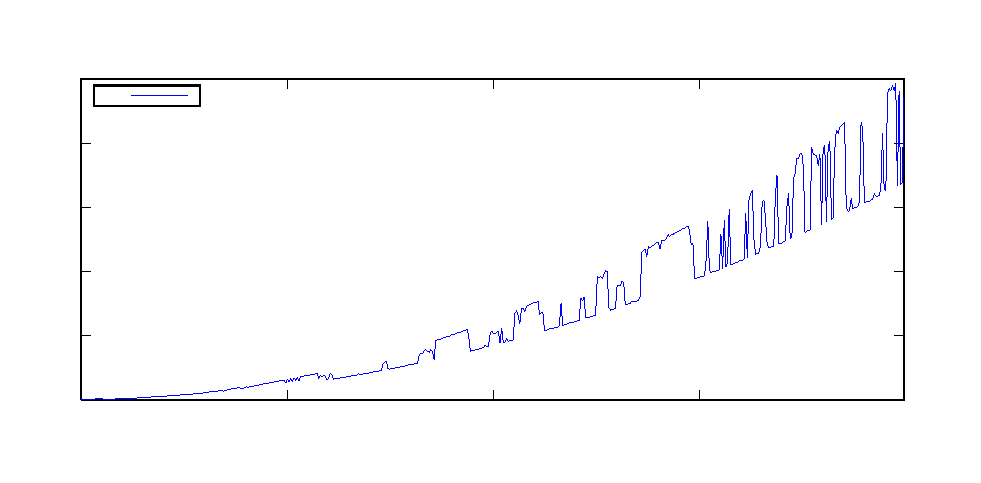
\includegraphics{problema3-mejor-caso}}%
    \gplfronttext
  \end{picture}%
\endgroup

  \caption{Mejor caso}
\end{figure}


\subsubsection{Instancias aleatorias}

\begin{figure}[H]
  \centering
  % GNUPLOT: LaTeX picture with Postscript
\begingroup
  \makeatletter
  \providecommand\color[2][]{%
    \GenericError{(gnuplot) \space\space\space\@spaces}{%
      Package color not loaded in conjunction with
      terminal option `colourtext'%
    }{See the gnuplot documentation for explanation.%
    }{Either use 'blacktext' in gnuplot or load the package
      color.sty in LaTeX.}%
    \renewcommand\color[2][]{}%
  }%
  \providecommand\includegraphics[2][]{%
    \GenericError{(gnuplot) \space\space\space\@spaces}{%
      Package graphicx or graphics not loaded%
    }{See the gnuplot documentation for explanation.%
    }{The gnuplot epslatex terminal needs graphicx.sty or graphics.sty.}%
    \renewcommand\includegraphics[2][]{}%
  }%
  \providecommand\rotatebox[2]{#2}%
  \@ifundefined{ifGPcolor}{%
    \newif\ifGPcolor
    \GPcolorfalse
  }{}%
  \@ifundefined{ifGPblacktext}{%
    \newif\ifGPblacktext
    \GPblacktexttrue
  }{}%
  % define a \g@addto@macro without @ in the name:
  \let\gplgaddtomacro\g@addto@macro
  % define empty templates for all commands taking text:
  \gdef\gplbacktext{}%
  \gdef\gplfronttext{}%
  \makeatother
  \ifGPblacktext
    % no textcolor at all
    \def\colorrgb#1{}%
    \def\colorgray#1{}%
  \else
    % gray or color?
    \ifGPcolor
      \def\colorrgb#1{\color[rgb]{#1}}%
      \def\colorgray#1{\color[gray]{#1}}%
      \expandafter\def\csname LTw\endcsname{\color{white}}%
      \expandafter\def\csname LTb\endcsname{\color{black}}%
      \expandafter\def\csname LTa\endcsname{\color{black}}%
      \expandafter\def\csname LT0\endcsname{\color[rgb]{1,0,0}}%
      \expandafter\def\csname LT1\endcsname{\color[rgb]{0,1,0}}%
      \expandafter\def\csname LT2\endcsname{\color[rgb]{0,0,1}}%
      \expandafter\def\csname LT3\endcsname{\color[rgb]{1,0,1}}%
      \expandafter\def\csname LT4\endcsname{\color[rgb]{0,1,1}}%
      \expandafter\def\csname LT5\endcsname{\color[rgb]{1,1,0}}%
      \expandafter\def\csname LT6\endcsname{\color[rgb]{0,0,0}}%
      \expandafter\def\csname LT7\endcsname{\color[rgb]{1,0.3,0}}%
      \expandafter\def\csname LT8\endcsname{\color[rgb]{0.5,0.5,0.5}}%
    \else
      % gray
      \def\colorrgb#1{\color{black}}%
      \def\colorgray#1{\color[gray]{#1}}%
      \expandafter\def\csname LTw\endcsname{\color{white}}%
      \expandafter\def\csname LTb\endcsname{\color{black}}%
      \expandafter\def\csname LTa\endcsname{\color{black}}%
      \expandafter\def\csname LT0\endcsname{\color{black}}%
      \expandafter\def\csname LT1\endcsname{\color{black}}%
      \expandafter\def\csname LT2\endcsname{\color{black}}%
      \expandafter\def\csname LT3\endcsname{\color{black}}%
      \expandafter\def\csname LT4\endcsname{\color{black}}%
      \expandafter\def\csname LT5\endcsname{\color{black}}%
      \expandafter\def\csname LT6\endcsname{\color{black}}%
      \expandafter\def\csname LT7\endcsname{\color{black}}%
      \expandafter\def\csname LT8\endcsname{\color{black}}%
    \fi
  \fi
  \setlength{\unitlength}{0.0500bp}%
  \begin{picture}(7678.00,5280.00)%
    \gplgaddtomacro\gplbacktext{%
      \colorrgb{0.00,0.00,0.00}%
      \put(740,640){\makebox(0,0)[r]{\strut{}$10^{0}$}}%
      \colorrgb{0.00,0.00,0.00}%
      \put(740,2660){\makebox(0,0)[r]{\strut{}$10^{1}$}}%
      \colorrgb{0.00,0.00,0.00}%
      \put(740,4679){\makebox(0,0)[r]{\strut{}$10^{2}$}}%
      \colorrgb{0.00,0.00,0.00}%
      \put(860,440){\makebox(0,0){\strut{}1x1,}}%
      \colorrgb{0.00,0.00,0.00}%
      \put(3012,440){\makebox(0,0){\strut{}2x2,}}%
      \colorrgb{0.00,0.00,0.00}%
      \put(5165,440){\makebox(0,0){\strut{}4x3,}}%
      \colorrgb{0.00,0.00,0.00}%
      \put(7317,440){\makebox(0,0){\strut{}5x5,}}%
      \colorrgb{0.00,0.00,0.00}%
      \put(160,2659){\rotatebox{90}{\makebox(0,0){\strut{}Tiempo de ejecuci\'on [$mS$]}}}%
      \colorrgb{0.00,0.00,0.00}%
      \put(4088,140){\makebox(0,0){\strut{}$n$ (tama\~no del problema)}}%
      \csname LTb\endcsname%
      \put(4088,4979){\makebox(0,0){\strut{}Instancias aleatorias}}%
    }%
    \gplgaddtomacro\gplfronttext{%
      \csname LTb\endcsname%
      \put(1220,4516){\makebox(0,0)[r]{\strut{}$t_n$}}%
    }%
    \gplbacktext
    \put(0,0){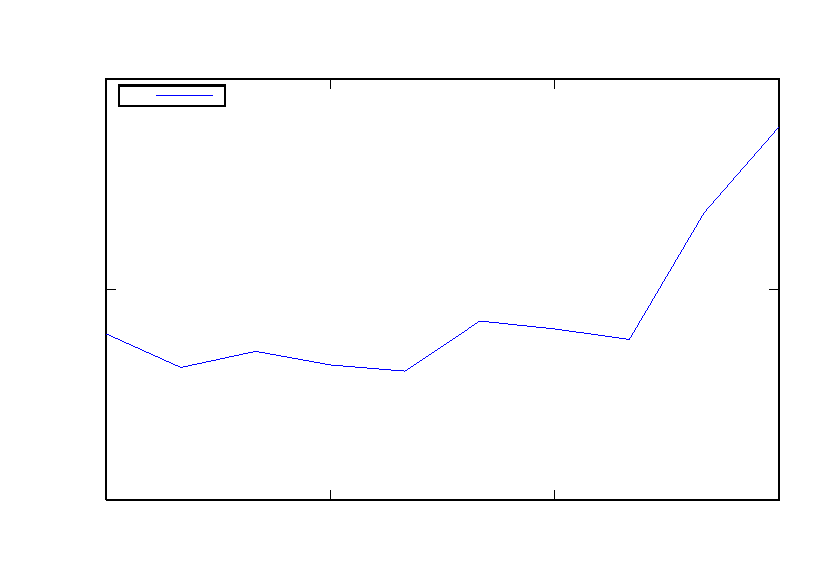
\includegraphics{problema3-instancias-aleatorias}}%
    \gplfronttext
  \end{picture}%
\endgroup

  \caption{Instancias aleatorias}
\end{figure}


%%%%%%%%%%%%%%%%%%%%%%%%%%%%%%%%%%%%%%%%%%%%%%%%%%%%%%%%%%%%%%%%%%%%%%%%%%%%%%%
%% Conclusiones                                                              %%
%%%%%%%%%%%%%%%%%%%%%%%%%%%%%%%%%%%%%%%%%%%%%%%%%%%%%%%%%%%%%%%%%%%%%%%%%%%%%%%


\newpage

\section{Conclusiones}

Pendiente.


%%%%%%%%%%%%%%%%%%%%%%%%%%%%%%%%%%%%%%%%%%%%%%%%%%%%%%%%%%%%%%%%%%%%%%%%%%%%%%%
%% Código fuente para el problema 1                                          %%
%%%%%%%%%%%%%%%%%%%%%%%%%%%%%%%%%%%%%%%%%%%%%%%%%%%%%%%%%%%%%%%%%%%%%%%%%%%%%%%


\newpage

\begin{appendices}

\section{Código fuente para el problema 1}

Pendiente.


%%%%%%%%%%%%%%%%%%%%%%%%%%%%%%%%%%%%%%%%%%%%%%%%%%%%%%%%%%%%%%%%%%%%%%%%%%%%%%%
%% Código fuente para el problema 1                                          %%
%%%%%%%%%%%%%%%%%%%%%%%%%%%%%%%%%%%%%%%%%%%%%%%%%%%%%%%%%%%%%%%%%%%%%%%%%%%%%%%


\newpage

\section{Código fuente para el problema 2}

Pendiente.


%%%%%%%%%%%%%%%%%%%%%%%%%%%%%%%%%%%%%%%%%%%%%%%%%%%%%%%%%%%%%%%%%%%%%%%%%%%%%%%
%% Código fuente para el problema 3                                          %%
%%%%%%%%%%%%%%%%%%%%%%%%%%%%%%%%%%%%%%%%%%%%%%%%%%%%%%%%%%%%%%%%%%%%%%%%%%%%%%%


\newpage

\section{Código fuente para el problema 3}

Pendiente.


\end{appendices}

\end{document}